%!TEX TS-program = xelatex
\documentclass[10pt,oneside]{article}
\usepackage[fontsize=9pt]{scrextend}

\usepackage[english]{babel}

\usepackage{amsmath,amssymb,amsfonts}
\usepackage[utf8]{inputenc}
\usepackage[T1]{fontenc}
\usepackage{stix2}
\usepackage[scaled]{helvet}
\usepackage[scaled]{inconsolata}

\usepackage{lastpage}

\usepackage{setspace}

\usepackage{ccicons}

\usepackage[hang,flushmargin]{footmisc}

\usepackage{geometry}

\setlength{\parindent}{0pt}
\setlength{\parskip}{6pt plus 2pt minus 1pt}

\usepackage{fancyhdr}
\renewcommand{\headrulewidth}{0pt}\providecommand{\tightlist}{%
  \setlength{\itemsep}{0pt}\setlength{\parskip}{0pt}}

\makeatletter
\newcounter{tableno}
\newenvironment{tablenos:no-prefix-table-caption}{
  \caption@ifcompatibility{}{
    \let\oldthetable\thetable
    \let\oldtheHtable\theHtable
    \renewcommand{\thetable}{tableno:\thetableno}
    \renewcommand{\theHtable}{tableno:\thetableno}
    \stepcounter{tableno}
    \captionsetup{labelformat=empty}
  }
}{
  \caption@ifcompatibility{}{
    \captionsetup{labelformat=default}
    \let\thetable\oldthetable
    \let\theHtable\oldtheHtable
    \addtocounter{table}{-1}
  }
}
\makeatother

\usepackage{array}
\newcommand{\PreserveBackslash}[1]{\let\temp=\\#1\let\\=\temp}
\let\PBS=\PreserveBackslash

\usepackage[breaklinks=true]{hyperref}
\hypersetup{colorlinks,%
citecolor=blue,%
filecolor=blue,%
linkcolor=blue,%
urlcolor=blue}
\usepackage{url}

\usepackage{caption}
\setcounter{secnumdepth}{0}
\usepackage{cleveref}

\usepackage{graphicx}
\makeatletter
\def\maxwidth{\ifdim\Gin@nat@width>\linewidth\linewidth
\else\Gin@nat@width\fi}
\makeatother
\let\Oldincludegraphics\includegraphics
\renewcommand{\includegraphics}[1]{\Oldincludegraphics[width=\maxwidth]{#1}}

\usepackage{longtable}
\usepackage{booktabs}

\usepackage{color}
\usepackage{fancyvrb}
\newcommand{\VerbBar}{|}
\newcommand{\VERB}{\Verb[commandchars=\\\{\}]}
\DefineVerbatimEnvironment{Highlighting}{Verbatim}{commandchars=\\\{\}}
% Add ',fontsize=\small' for more characters per line
\usepackage{framed}
\definecolor{shadecolor}{RGB}{248,248,248}
\newenvironment{Shaded}{\begin{snugshade}}{\end{snugshade}}
\newcommand{\KeywordTok}[1]{\textcolor[rgb]{0.13,0.29,0.53}{\textbf{#1}}}
\newcommand{\DataTypeTok}[1]{\textcolor[rgb]{0.13,0.29,0.53}{#1}}
\newcommand{\DecValTok}[1]{\textcolor[rgb]{0.00,0.00,0.81}{#1}}
\newcommand{\BaseNTok}[1]{\textcolor[rgb]{0.00,0.00,0.81}{#1}}
\newcommand{\FloatTok}[1]{\textcolor[rgb]{0.00,0.00,0.81}{#1}}
\newcommand{\ConstantTok}[1]{\textcolor[rgb]{0.00,0.00,0.00}{#1}}
\newcommand{\CharTok}[1]{\textcolor[rgb]{0.31,0.60,0.02}{#1}}
\newcommand{\SpecialCharTok}[1]{\textcolor[rgb]{0.00,0.00,0.00}{#1}}
\newcommand{\StringTok}[1]{\textcolor[rgb]{0.31,0.60,0.02}{#1}}
\newcommand{\VerbatimStringTok}[1]{\textcolor[rgb]{0.31,0.60,0.02}{#1}}
\newcommand{\SpecialStringTok}[1]{\textcolor[rgb]{0.31,0.60,0.02}{#1}}
\newcommand{\ImportTok}[1]{#1}
\newcommand{\CommentTok}[1]{\textcolor[rgb]{0.56,0.35,0.01}{\textit{#1}}}
\newcommand{\DocumentationTok}[1]{\textcolor[rgb]{0.56,0.35,0.01}{\textbf{\textit{#1}}}}
\newcommand{\AnnotationTok}[1]{\textcolor[rgb]{0.56,0.35,0.01}{\textbf{\textit{#1}}}}
\newcommand{\CommentVarTok}[1]{\textcolor[rgb]{0.56,0.35,0.01}{\textbf{\textit{#1}}}}
\newcommand{\OtherTok}[1]{\textcolor[rgb]{0.56,0.35,0.01}{#1}}
\newcommand{\FunctionTok}[1]{\textcolor[rgb]{0.00,0.00,0.00}{#1}}
\newcommand{\VariableTok}[1]{\textcolor[rgb]{0.00,0.00,0.00}{#1}}
\newcommand{\ControlFlowTok}[1]{\textcolor[rgb]{0.13,0.29,0.53}{\textbf{#1}}}
\newcommand{\OperatorTok}[1]{\textcolor[rgb]{0.81,0.36,0.00}{\textbf{#1}}}
\newcommand{\BuiltInTok}[1]{#1}
\newcommand{\ExtensionTok}[1]{#1}
\newcommand{\PreprocessorTok}[1]{\textcolor[rgb]{0.56,0.35,0.01}{\textit{#1}}}
\newcommand{\AttributeTok}[1]{\textcolor[rgb]{0.77,0.63,0.00}{#1}}
\newcommand{\RegionMarkerTok}[1]{#1}
\newcommand{\InformationTok}[1]{\textcolor[rgb]{0.56,0.35,0.01}{\textbf{\textit{#1}}}}
\newcommand{\WarningTok}[1]{\textcolor[rgb]{0.56,0.35,0.01}{\textbf{\textit{#1}}}}
\newcommand{\AlertTok}[1]{\textcolor[rgb]{0.94,0.16,0.16}{#1}}
\newcommand{\ErrorTok}[1]{\textcolor[rgb]{0.64,0.00,0.00}{\textbf{#1}}}
\newcommand{\NormalTok}[1]{#1}

\newlength{\cslhangindent}
\setlength{\cslhangindent}{1.5em}
\newlength{\csllabelwidth}
\setlength{\csllabelwidth}{3em}
\newenvironment{CSLReferences}[3] % #1 hanging-ident, #2 entry spacing
 {% don't indent paragraphs
  \setlength{\parindent}{0pt}
  % turn on hanging indent if param 1 is 1
  \ifodd #1 \everypar{\setlength{\hangindent}{\cslhangindent}}\ignorespaces\fi
  % set entry spacing
  \ifnum #2 > 0
  \setlength{\parskip}{#2\baselineskip}
  \fi
 }%
 {}
\usepackage{calc} % for \widthof, \maxof
\newcommand{\CSLBlock}[1]{#1\hfill\break}
\newcommand{\CSLLeftMargin}[1]{\parbox[t]{\maxof{\widthof{#1}}{\csllabelwidth}}{#1}}
\newcommand{\CSLRightInline}[1]{\parbox[t]{\linewidth}{#1}}
\newcommand{\CSLIndent}[1]{\hspace{\cslhangindent}#1}\usepackage[table,dvipsnames]{xcolor}

\geometry{includemp,
            letterpaper,
            top=1.0in,
            bottom=2.510cm,
            left=0.35in,
            right=0.35in,
            marginparwidth=2.0in,
            marginparsep=0.35in}

\usepackage[singlelinecheck=off]{caption}
\captionsetup{
  font={small},
  labelfont={bf},
  format=plain,
  labelsep=quad
}

\usepackage{floatrow}

\floatsetup[figure]{margins=hangright,
              facing=no,
              capposition=beside,
              capbesideposition={center,outside},
              floatwidth=\textwidth}

% \floatsetup[table]{margins=hangright,
%              facing=no,
%              capposition=beside,
%              capbesideposition={center,outside},
%              floatwidth=\textwidth}

\pagestyle{plain}

\setcounter{secnumdepth}{5}

\usepackage{titlesec}

\titleformat{\section}[block]
{\normalfont\large\sffamily}
{\thesection}{.5em}{\titlerule\\[.8ex]\bfseries}

\titleformat{\subsection}[runin]
{\normalfont\fontseries{b}\selectfont\filright\sffamily}
{\thesubsection.}{.5em}{}

\titleformat{\subsubsection}[runin]
{\normalfont\itshape\rmfamily\bfseries}{\thesubsubsection}{1em}{}

\fancypagestyle{firstpage}
{
   \fancyhf{}
   \renewcommand{\headrulewidth}{0pt}
   \fancyfoot[R]{\footnotesize\ccby}
   \fancyfoot[L]{\footnotesize\sffamily\today}
}

\fancypagestyle{normal}
{
  \fancyhf{}
  \fancyfoot[R]{\footnotesize\sffamily\thepage\ of \pageref*{LastPage}}
}

\usepackage{tikz}
\begin{document}
\tikz [remember picture, overlay] %
\node [shift={(-0.6in,1.1cm)},scale=0.2,opacity=0.4] at (current page.south east)[anchor=south east]{
\includegraphics{logo}};%
\pagestyle{normal}
\thispagestyle{firstpage}

\newcommand{\colorRule}[3][black]{\textcolor[HTML]{#1}{\rule{#2}{#3}}}

\noindent {\LARGE \textbf{\textsf{Food web reconstruction through
phylogenetic transfer of low-rank network representation}}}

\medskip
\begin{flushleft}
{\small
%
\href{https://orcid.org/0000-0001-6067-1349}{Tanya\,Strydom}%
%
\,\textsuperscript{1,2,‡}, %
\href{https://orcid.org/0000-0003-0193-5441}{Salomé\,Bouskila}%
%
\,\textsuperscript{1,‡}, %
\href{https://orcid.org/0000-0001-9051-0597}{Francis\,Banville}%
%
\,\textsuperscript{1,3,2}, %
\href{https://orcid.org/0000-0003-4036-977X}{Ceres\,Barros}%
%
\,\textsuperscript{4}, %
\href{https://orcid.org/0000-0002-2151-6693}{Dominique\,Caron}%
%
\,\textsuperscript{5,2}, %
\href{https://orcid.org/0000-0003-0452-6993}{Maxwell J\,Farrell}%
%
\,\textsuperscript{6}, %
\href{https://orcid.org/0000-0002-9935-1366}{Marie-Josée\,Fortin}%
%
\,\textsuperscript{6}, %
\href{https://orcid.org/0000-0003-3220-6161}{Victoria\,Hemming}%
%
\,\textsuperscript{4}, %
\href{https://orcid.org/0000-0002-4104-9463}{Benjamin\,Mercier}%
%
\,\textsuperscript{3,2}, %
\href{https://orcid.org/0000-0002-6004-4027}{Laura J.\,Pollock}%
%
\,\textsuperscript{5,2}, %
\href{https://orcid.org/0000-0001-5785-8321}{Rogini\,Runghen}%
%
\,\textsuperscript{7}, %
\href{https://orcid.org/0000-0002-3454-0633}{Giulio V.\,Dalla Riva}%
%
\,\textsuperscript{8}, %
\href{https://orcid.org/0000-0002-0735-5184}{Timothée\,Poisot}%
%
\,\textsuperscript{1,2}
\vskip 1em
\textsuperscript{1}\,Département de Sciences Biologiques, Université de
Montréal, Montréal, Canada; \textsuperscript{2}\,Québec Centre for
Biodiversity Sciences, Montréal, Canada; \textsuperscript{3}\,Université
de Sherbrooke, Sherbrooke, Canada; \textsuperscript{4}\,Department of
Forest Resources Management, University of British Columbia, Vancouver,
Canada; \textsuperscript{5}\,Department of Biology, McGill University,
Montréal, Canada; \textsuperscript{6}\,Department of Ecology \&
Evolutionary Biology, University of Toronto, Toronto,
Canada; \textsuperscript{7}\,Centre for Integrative Ecology, School of
Biological Sciences, University of Canterbury, Canterbury, New
Zealand; \textsuperscript{8}\,School of Mathematics and Statistics,
University of Canterbury, Canterbury, New Zealand\\
\textsuperscript{‡}\,These authors contributed equally to the work\\
\vskip 1em
\textbf{Correspondance to:}\\
Timothée Poisot --- \texttt{timothee.poisot@umontreal.ca}\\
}
\end{flushleft}

\vskip 2em
\makebox[0pt][l]{\colorRule[CCCCCC]{2.0\textwidth}{0.5pt}}
\vskip 2em
\noindent

\marginpar{\vskip 1em\flushright
{\small{\bfseries Keywords}:\par
ecological networks\\network embedding\\transfer learning\\ancestral
character estimation\\biogeography\\}
}


Despite their importance in many ecological processes, collecting data
and information on ecological interactions, and therefore species
interaction networks, is an exceedingly challenging task. For this
reason, large parts of the world have a data deficit when it comes to
species interactions, and how the resulting networks are structured. As
data collection alone is unlikely to be sufficient at filling these
global gaps, community ecologists must adopt predictive methods. In this
contribution, we develop such a method, relying on graph embedding (the
extraction of explanatory latent variables from known graph structures)
and transfer learning (the application of previous solutions to novel
problems with limited predictors overlap) in order to assemble a
predicted list of trophic interactions between mammals of Canada. This
interaction list is derived from extensive knowledge of the mammalian
food web of Europe, despite the fact that there are fewer than 5\% of
common species between the two locations. The results of the predictive
model are compared against databases of recorded pairwise interactions,
showing that we correctly recover over 95\% of known interactions. We
provide guidance on how this method can be adapted by substituting some
approaches or predictors in order to make it more generally applicable.




\vskip 2em
\makebox[0pt][l]{\colorRule[CCCCCC]{2.0\textwidth}{0.5pt}}
\vskip 2em

\hypertarget{introduction}{%
\section{Introduction}\label{introduction}}

There are two core challenges we are faced with in furthering our
understanding of ecological networks across space, particularly at
macro-ecologically relevant scales (\emph{e.g.} Trøjelsgaard \& Olesen
2016). First, networks within a location are difficult to sample
properly (Jordano 2016a, b), resulting in a widespread ``Eltonian
shortfall'' (Hortal \emph{et al.} 2015), \emph{i.e.} a lack of knowledge
about inter and intra specific relationships. This first challenge has
been, in large part, addressed by the recent emergence of a suite of
methods aiming to predict interactions within \emph{existing} networks,
many of which are reviewed in Strydom \emph{et al.} (2021a). Second,
recent analyses based on collected data (Poisot \emph{et al.} 2021a) or
metadata (Cameron \emph{et al.} 2019) highlight that ecological networks
are currently studied in a biased subset of space and bioclimates, which
impedes our ability to generalize any local understanding of network
structure. Meaning that, although the framework to address
incompleteness \emph{within} networks exists, there would still be
regions for which, due to a \emph{lack} of local interaction data, we
are unable to infer potential species interactions. Having a general
solution for inferring a \emph{plausible} metaweb (despite the
unavailability of interaction data) could be the catalyst for
significant breakthroughs in our ability to start thinking about species
interactions networks over large spatial scales.

Here, we present a general method for the transfer learning of network
representations, relying on the similarities of species in a
biologically/ecologically relevant proxy space (\emph{e.g.} shared
morphology or ancestry). Transfer learning is a machine learning
methodology that uses the knowledge gained from solving one problem and
applying it to a related (destination) problem (Pan \& Yang 2010; Torrey
\& Shavlik 2010). In this instance, we solve the problem of predicting
trophic interactions between species, based on knowledge extracted from
another species pool for which interactions are known by using
phylogenetic structure as a medium for transfer. This allows us to
construct a \emph{probabilistic} metaweb for a community for which we
have \emph{no} prior trophic interaction data for the desired species
pool. Our methodology is outlined in fig.~\ref{fig:concept}, where we
provide an illustration based on learning the embedding of a metaweb of
trophic interactions for European mammals (known interactions; Maiorano
\emph{et al.} 2020b, a) and, based on phylogenetic relationships between
mammals globally (\emph{i.e.}, phylogenetic tree Upham \emph{et al.}
2019), infer a metaweb for the Canadian mammalian species pool
(interactions are treated as unknown in this instance).

\begin{figure}
\hypertarget{fig:concept}{%
\centering
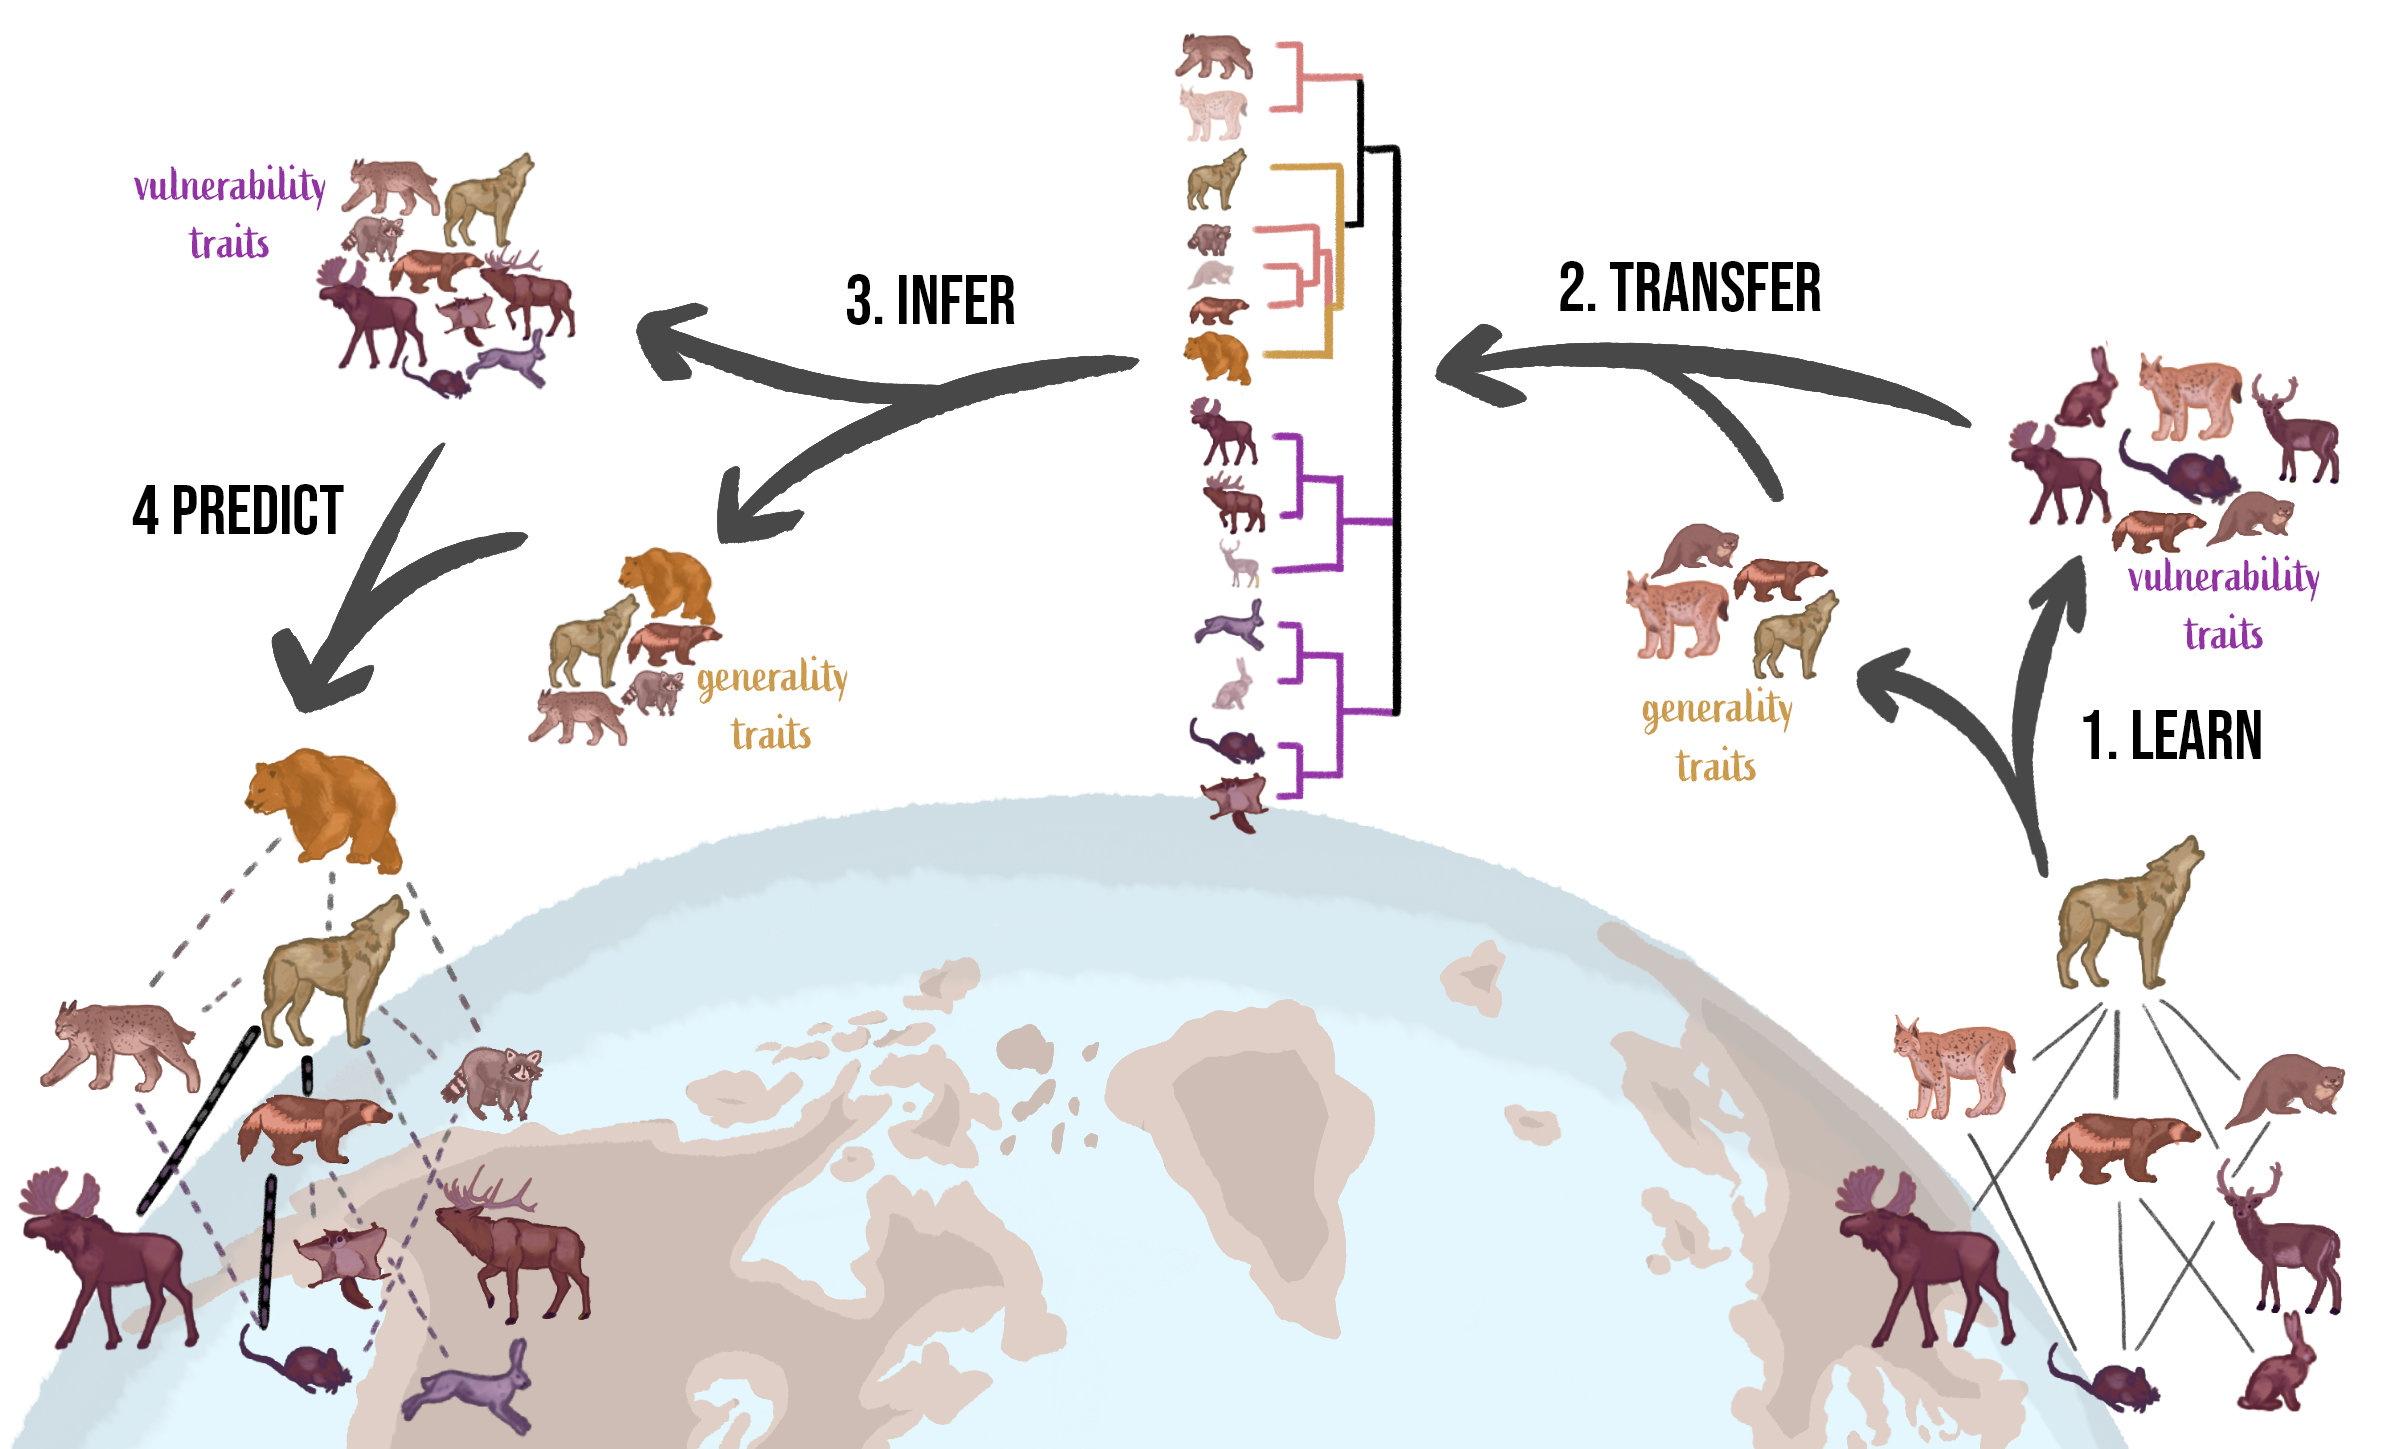
\includegraphics{figures/figure-concept.png}
\caption{Overview of the phylogenetic transfer learning (and prediction)
of species interactions networks. Starting from an initial, known,
network, we learn its representation through a graph embedding step
(here, a truncated Singular Value Decomposition; Step 1), yielding a
series of latent traits (vulnerability traits representing species at
the lower trophic-level and generality traits representing species at
higher trophic-levels; \emph{sensu} Schoener (1989)); second, for the
destination species pool, we perform ancestral character estimation
using a phylogeny (here, using a Brownian model for the latent traits;
Step 2); we then sample from the reconstructed distribution of latent
traits (Step 3) to generate a probabilistic metaweb at the destination
(here, assuming a uniform distribution of traits), and threshold it to
yield the final list of interactions (Step 4).}\label{fig:concept}
}
\end{figure}

There is a plurality of measures of species similarities that can be
used for metaweb reconstruction (see \emph{e.g.} Morales-Castilla
\emph{et al.} 2015); however, phylogenetic proximity has several
desirable properties when working at large scales. Gerhold \emph{et al.}
(2015) made the point that phylogenetic signal captures diversification
of characters (large macro-evolutionary process), but not necessarily
community assembly (fine ecological process); Dormann \emph{et al.}
(2010) previously found very similar conclusions. Interactions tend
reflect a phylogenetic signal because they have a conserved pattern of
evolutionary convergence that encompasses a wide range of ecological and
evolutionary mechanisms (Cavender-Bares \emph{et al.} 2009; Mouquet
\emph{et al.} 2012), and - most importantly - retain this signal even
when it is not detectable at the community scale (Hutchinson \emph{et
al.} 2017; Poisot \& Stouffer 2018). Finally, species interactions at
macro-ecological scales seem to respond mostly to macro-evolutionary
processes (Price 2003); which is evidenced by the presence of conserved
backbones in food webs (Dalla Riva \& Stouffer 2016), strong
evolutionary signature on prey choice (Stouffer \emph{et al.} 2012), and
strong phylogenetic signature in food web intervality (Eklöf \& Stouffer
2016). Phylogenetic reconstruction has also previously been used within
the context of ecological networks, namely understanding ancestral
plant-insect interactions (Braga \emph{et al.} 2021). Taken together,
these considerations suggest that phylogenies can reliably be used to
transfer knowledge on species interactions.

Our case study shows that phylogenetic transfer learning is indeed an
effective approach to predict the Canadian mammalian metaweb. This
showcases that although the components (species) that make up the
Canadian and European communities may be \emph{minimally} shared, if the
medium (proxy space) selected in the transfer step is biologically
plausible, we can still effectively learn from the known network and
make biologically relevant predictions of interactions. It should be
reiterated that the framework presented in fig.~\ref{fig:concept} is
amenable to changes; notably, the measure of similarity may not be
phylogeny, and can be replaced by information on foraging (Beckerman
\emph{et al.} 2006), cell-level mechanisms (Boeckaerts \emph{et al.}
2021), or a combination of traits and phylogenetic structure (Stock
2021).

\hypertarget{data-used-for-the-case-study}{%
\section{Data used for the case
study}\label{data-used-for-the-case-study}}

We use data from the European metaweb assembled by Maiorano \emph{et
al.} (2020b), following the definition of the metaweb first introduced
by Dunne (2006), \emph{i.e.} an inventory of all possible interactions
within species from a spatially delimited pool. Notably the metaweb is
not a prediction of the food web at any specific locale within the
frontiers of the species pool -- in fact, these local food webs are
expected to have a subset of both the species and the interactions of
their metaweb (Poisot \emph{et al.} 2012). This being said, as the
metaweb represents the total of functional, phylogenetic, and
macroecological processes (Morales-Castilla \emph{et al.} 2015), it is
thus still worthy of ecological attention. We deduced the subgraph
corresponding to all mammals by matching species names in the original
network to the GBIF taxonomic backbone (GBIF Secretariat 2021) and
retaining all those who matched to mammals. This serves a dual purpose
1) to extract only mammals from the European network and 2) to match and
standardize species names when aggregating the different data sources
further downstream (which is an important consideration when combining
datasets Grenié \emph{et al.} (2021)). All nodes had valid matches to
GBIF at this step, and so this backbone is used for all name
reconciliation steps as outlined below.

The European metaweb represents the knowledge we want to learn and
transfer; the phylogenetic similarity of mammals here represents the
information for transfer. We used the mammalian consensus supertree by
Upham \emph{et al.} (2019), for which all approximatively 6000 names
have been similarly matched to their GBIF valid names. This step allows
us to place each node of the mammalian European metaweb in the
phylogeny.

The destination problem to which we want to transfer knowledge is the
trophic interactions between mammals in Canada. We obtained the list of
extant species from the IUCN checklist, and selected the terrestrial and
semi-aquatic species (this corresponds to the same selection that was
applied by Maiorano \emph{et al.} (2020b) in the European metaweb). The
IUCN names were, as previously, reconciled against GBIF to have an exact
match to the taxonomy.

After taxonomic cleaning and reconciliation as outlined in the following
sections, the mammalian European metaweb has 260 species, and the
Canadian species pool has 163; of these, 17 (about 4\% of the total) are
shared, and 89 species from Canada (54\%) had at least one congeneric
species in Europe. The similarity for both species pools predictably
increases with higher taxonomic order, with 19\% of shared genera, 47\%
of shared families, and 75\% of shared orders; for the last point,
Canada and Europe each had a single unique order (\emph{Didelphimorphia}
for Canada, \emph{Erinaceomorpha} for Europe).

In the following sections, we describe the representational learning
step applied to European data, the transfer step through phylogenetic
similarity, and the generation of a probabilistic metaweb for the
destination species pool.

\hypertarget{method-description}{%
\section{Method description}\label{method-description}}

The crux of the method is the transfer of knowledge of a known network,
in order to predict interactions between species from another location.
In fig.~\ref{fig:concept}, we give a high-level overview of the
approach; in the example around which this manuscript is built
(leveraging detailed knowledge about binary trophic interactions between
Mammalia in Europe to predict the less known trophic interactions
between closely phylogenetically related Mammalia in Canada), we use a
series of specific steps for network embedding, trait inference, network
prediction and thresholding.

Specifically, our approach can be summarized as follows: from the known
network in Europe, we use a truncated Singular Value Decomposition
(t-SVD; Halko \emph{et al.} 2011) to generate latent traits representing
a low-dimensional embedding of the network; these traits give an
unbiased estimate of the node's position in the latent feature spaces.
Then, we map these latent traits onto a reference phylogeny (other
distance-based measures of species proximity that allow for the
inference of features in the latent space can be used, for example the
dissimilarity in functional traits). Based on the reconstructed latent
traits for species in the destination species pool, a Random Dot Product
Graph model (hereafter RDPG; Young \& Scheinerman 2007) predicts the
interaction between species through a function of the nodes' features
through matrix multiplication. Thus, from latent traits and node
position, we can infer interactions.

\hypertarget{implementation-and-code-availability}{%
\subsection{Implementation and code
availability}\label{implementation-and-code-availability}}

The entire pipeline is implemented in \emph{Julia} 1.6 (Bezanson
\emph{et al.} 2017) and is available under the permissive MIT License at
\href{https://osf.io/2zwqm/}{\texttt{https://osf.io/2zwqm/}}. The
taxonomic cleanup steps are done using \texttt{GBIF.jl} (Dansereau \&
Poisot 2021). The network embedding and analysis is done using
\texttt{EcologicalNetworks.jl} (Poisot \emph{et al.} 2019; Banville
\emph{et al.} 2021). The phylogenetic simulations are done using
\texttt{PhyloNetworks.jl} (Solís-Lemus \emph{et al.} 2017) and
\texttt{Phylo.jl} (Reeve \emph{et al.} 2016). A complete
\texttt{Project.toml} file specifying the full tree of dependencies is
available alongside the code. This material also includes a fully
annotated copy of the entire code required to run this project
(describing both the intent of the code and discussing some technical
implementation details), a vignette for every step of the process, and a
series of Jupyter notebooks with the text and code. The pipeline can be
executed on a laptop in a matter of minutes, and therefore does not
require extensive computational power.

\hypertarget{step-1-learning-the-origin-network-representation}{%
\subsection{Step 1: Learning the origin network
representation}\label{step-1-learning-the-origin-network-representation}}

The first step in transfer learning is to learn the structure of the
original dataset. In order to do so, we rely on an approach inspired
from representational learning, where we learn a \emph{representation}
of the metaweb (in the form of the latent subspaces), rather than a list
of interactions (species \emph{a} eats \emph{b}). This approach is
conceptually different from other metaweb-scale predictions (\emph{e.g.}
Albouy \emph{et al.} 2019), in that the metaweb representation is easily
transferable. Specifically, we use RDPG to create a number of latent
variables that can be combined into an approximation of the network
adjacency matrix. RDPG results are known to have strong phylogenetic
signal, and to capture the evolutionary backbone of food webs (Dalla
Riva \& Stouffer 2016). In addition, recent advances show that the
latent variables produced this way can be used to predict \emph{de novo}
network edges (\emph{i.e.} interactions; Runghen \emph{et al.} 2021).

The latent variables are created by performing a truncated Singular
Value Decomposition (t-SVD) on the adjacency matrix. SVD is an
appropriate embedding of ecological networks, which has recently been
shown to both capture their complex, emerging properties (Strydom
\emph{et al.} 2021b) and to allow highly accurate prediction of the
interactions within a single network (Poisot \emph{et al.} 2021b). Under
SVD, an adjacency matrix \(\mathbf{A}\) (where
\(\mathbf{A}_{m,n}\in\mathbb{B}\) where 1 indicates predation and 0 an
absence thereof) is decomposed into three components resulting in
\(\mathbf{A} = \mathbf{L}\mathbf{\Sigma}\mathbf{R'}.\) Here,
\(\mathbf{\Sigma}\) is a \(m \times n\) diagonal matrix and contains
only singular (\(\sigma\)) values along its diagonal, \(\mathbf{L}\) is
a \(m \times m\) unitary matrix, and \(\mathbf{R}'\) a \(n \times n\)
unitary matrix. Truncating the SVD removes additional noise in the
dataset by omitting non-zero and/or smaller \(\sigma\) values from
\(\mathbf{\Sigma}\) using the rank of the matrix. Under a t-SVD
\(\mathbf{A}_{m,n}\) is decomposed so that \(\mathbf{\Sigma}\) is a
square \(r \times r\) diagonal matrix (whith \(1 \le r \le r_{full}\)
where \(r_{full}\) is the full rank of \(\mathbf{A}\) and \(r\) the rank
at which we truncate the matrix) containing only non-zero \(\sigma\)
values. Additionally, \(\mathbf{L}\) is now a \(m \times r\) semi
unitary matrix and \(\mathbf{R}'\) a \(n \times r\) semi-unitary matrix.

The specific rank at which the SVD ought to be truncated is a difficult
question. The purpose of SVD is to remove the noise (expressed at high
dimensions) and to focus on the signal, (expressed at low dimensions).
In datasets with a clear signal/noise demarcation, a scree plot of
\(\mathbf{\Sigma}\) can show a sharp drop at the rank where noise starts
(Zhu \& Ghodsi 2006). Because the European metaweb is almost entirely
known, the amount of noise (uncertainty) is low; this is reflected in
fig.~\ref{fig:scree} (left), where the scree plot shows no important
drop, and in fig.~\ref{fig:scree} (right) where the proportion of
variance explained increases smoothly at higher dimensions. For this
reason, we default back to a threshold that explains 60\% of the
variance in the underlying data, corresponding to 12 dimensions -
\emph{i.e.} a tradeoff between accuracy and a reduced number of
features.

A RDPG estimates the probability of observing interactions between nodes
(species) as a function of the nodes' latent variables. The latent
variables used for the RDPG, called the left and right subspaces, are
defined as \(\mathcal{L} = \mathbf{L}\sqrt{\mathbf{\Sigma}}\), and
\(\mathcal{R} = \sqrt{\mathbf{\Sigma}}\mathbf{R}\) -- using the full
rank of \(\mathbf{A}\), \(\mathcal{L}\mathcal{R}' = \mathbf{A}\), and
using any smaller rank results in
\(\mathcal{L}\mathcal{R}' \approx \mathbf{A}\). Using a rank of 1 for
the t-SVD provides a first-order approximation of the network.

\begin{figure}
\hypertarget{fig:scree}{%
\centering
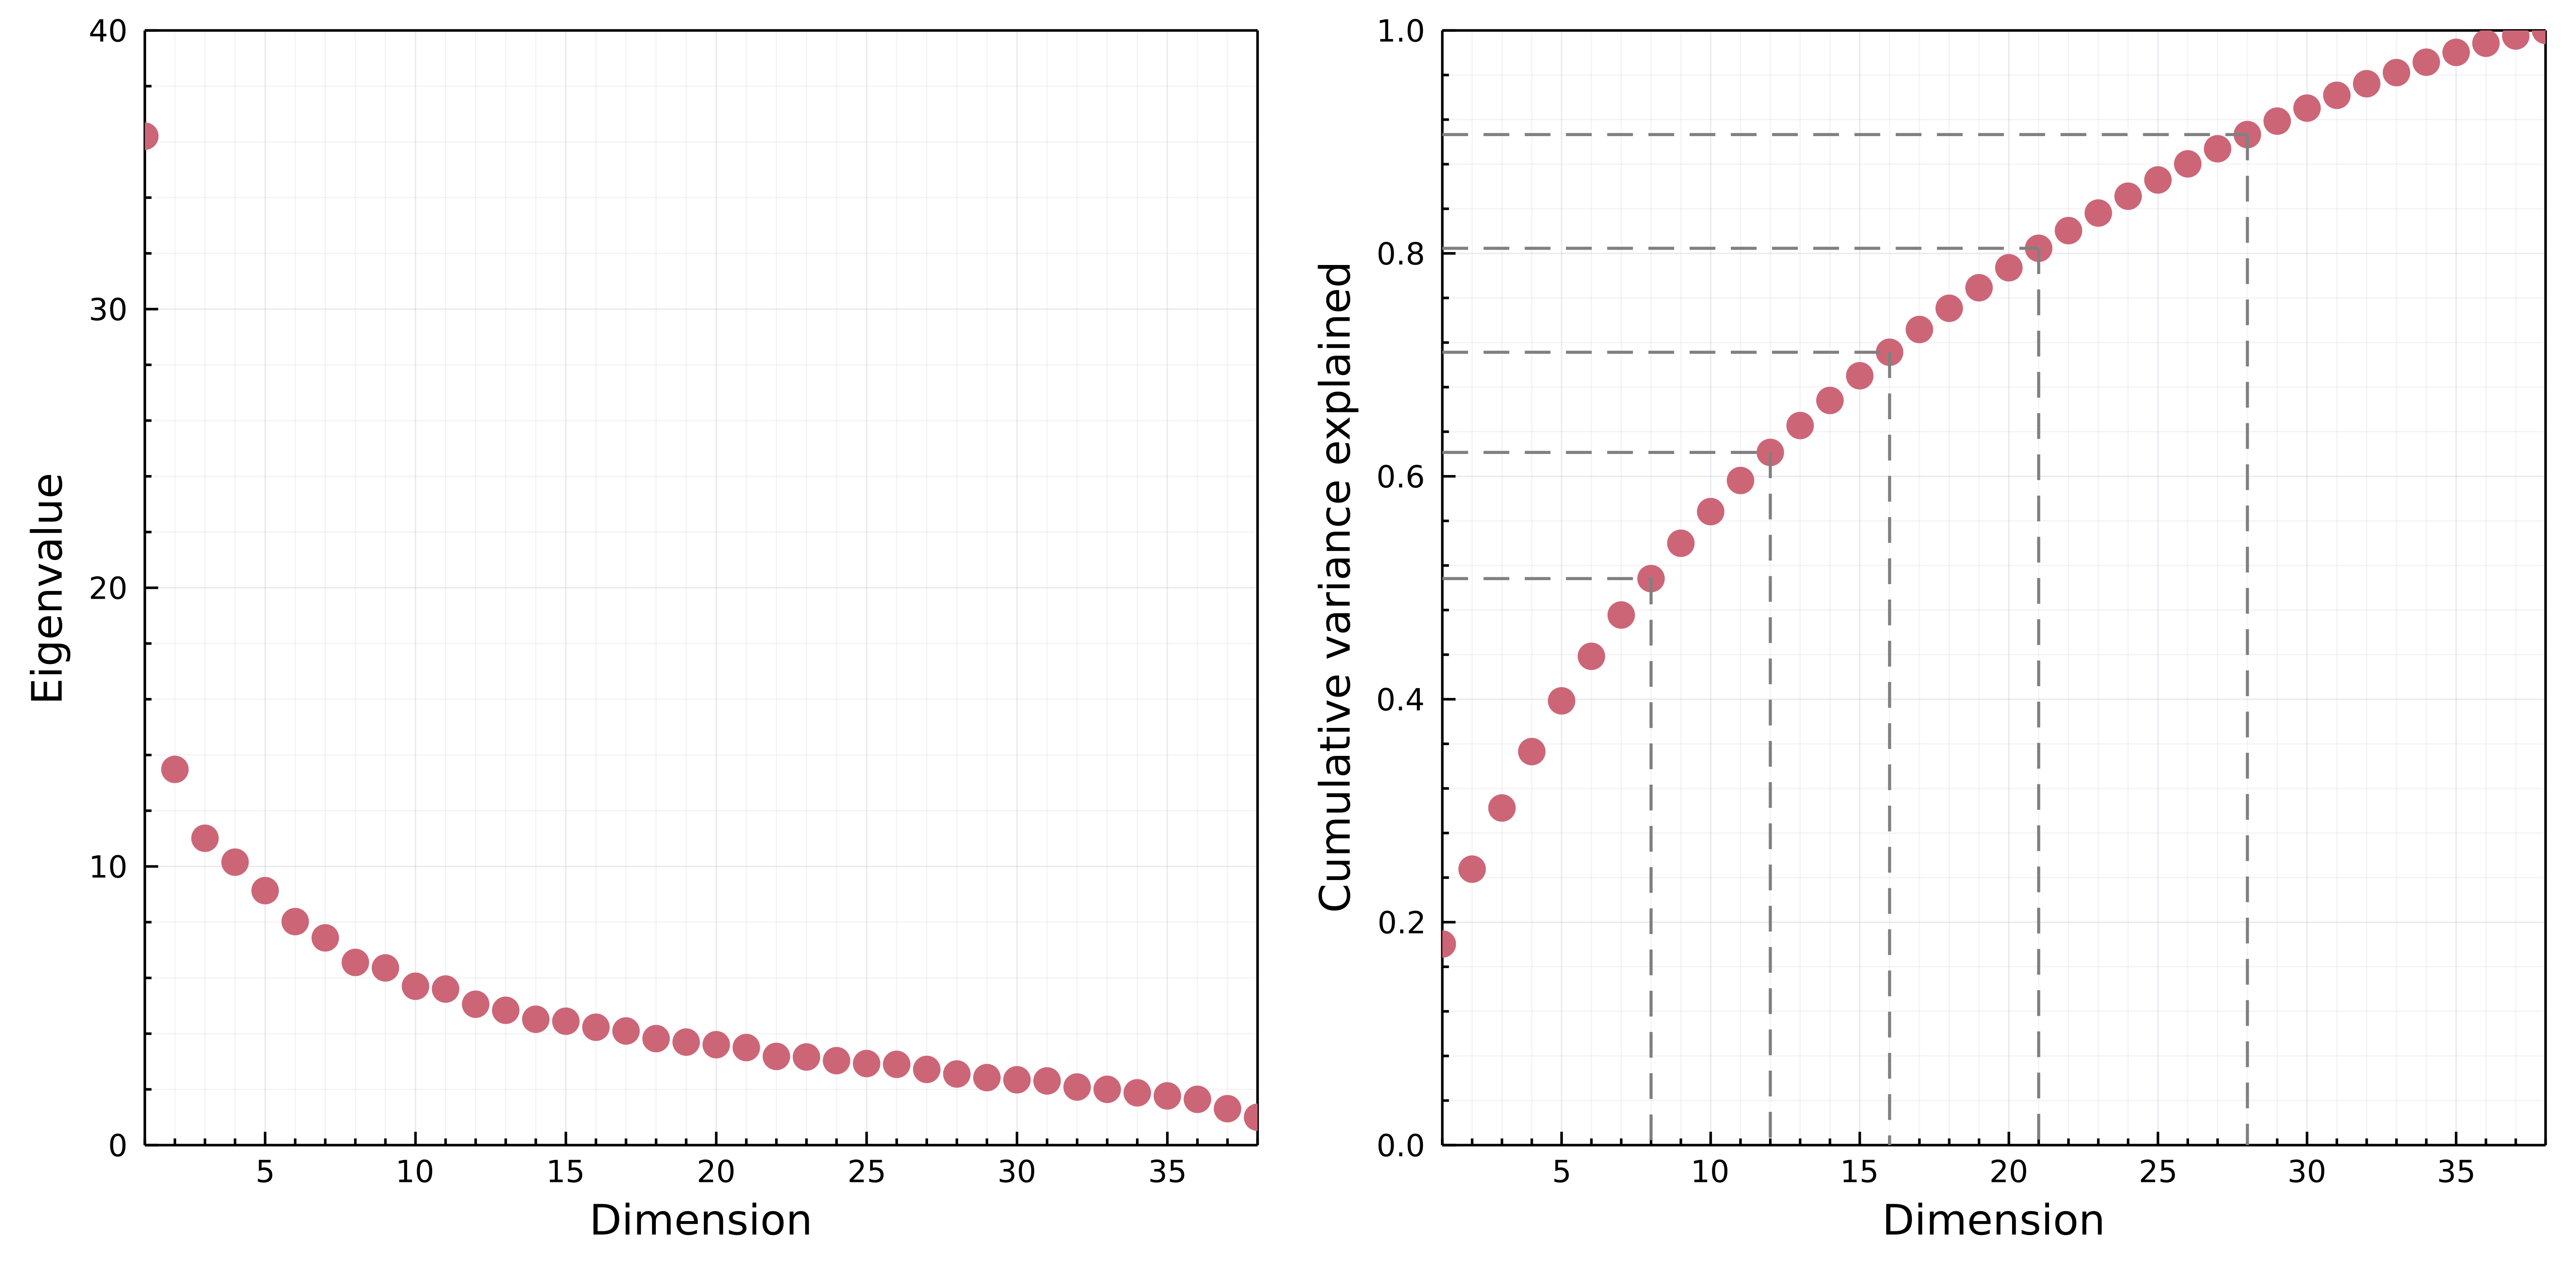
\includegraphics{figures/figure-screeplot.png}
\caption{Left: representation of the screeplot of the singular values
from the t-SVD on the European metaweb. The screeplot shows no obvious
drop in the singular values that may be leveraged to automatically
detect a minimal dimension for embedding, after \emph{e.g.} Zhu \&
Ghodsi (2006). Right: cumulative fraction of variance explained by each
dimension up to the rank of the European metaweb. The grey lines
represent cutoffs at 50, 60\ldots{} 90\% of variance explained. For the
rest of the analysis, we reverted to an arbitrary threshold of 60\% of
variance explained, which represented a good tradeoff between accuracy
and reduced number of features.}\label{fig:scree}
}
\end{figure}

Because RDPG relies on matrix multiplication, the higher dimensions
essentially serve to make specific interactions converge towards 0 or 1;
therefore, for reasonably low ranks, there is no guarantee that the
values in the reconstructed network will be within the unit range. In
order to determine what constitutes an appropriate threshold for
probability, we performed the RDPG approach on the European metaweb, and
evaluated the probability threshold by treating this as a binary
classification problem, specifically assuming that both 0 and 1 in the
European metaweb are all true. Given the methodological details given in
Maiorano \emph{et al.} (2020b) and O'Connor \emph{et al.} (2020), this
seems like a reasonable assumption, although one that does not hold for
all metawebs. We used the thresholding approach presented in Poisot
\emph{et al.} (2021b), and picked a cutoff that maximized Youden's \(J\)
statistic (a measure of the informedness (trust) of predictions; Youden
(1950)); the resulting cutoff was 0.22, and gave an accuracy above 0.99.

The left and right subspaces for the European metaweb, accompanied by
the threshold for prediction, represent the knowledge we seek to
transfer. In the next section, we explain how we rely on phylogenetic
similarity to do so.

\hypertarget{steps-2-and-3-transfer-learning-through-phylogenetic-relatedness}{%
\subsection{Steps 2 and 3: Transfer learning through phylogenetic
relatedness}\label{steps-2-and-3-transfer-learning-through-phylogenetic-relatedness}}

In order to transfer the knowledge from the European metaweb to the
Canadian species pool, we performed ancestral character estimation using
a Brownian motion model, which is a conservative approach in the absence
of strong hypotheses about the nature of phylogenetic signal in the
network decomposition (Litsios \& Salamin 2012). This uses the estimated
feature vectors for the European mammals to create a state
reconstruction for all species (conceptually something akin to a
trait-based mammalian phylogeny using generality and vulnerability
traits) and allows us to impute the missing (latent) trait data for the
Canadian species that are not already in the European network; as we are
focused on predicting contemporary interactions, we only retained the
values for the tips of the tree. We assumed that all traits (\emph{i.e.}
the feature vectors for the left and right subspaces) were independent,
which is a reasonable assumption as every trait/dimension added to the
t-SVD has an \emph{additive} effect to the one before it. Note that the
Upham \emph{et al.} (2019) tree itself has some uncertainty associated
to inner nodes of the phylogeny. In this case study, we have decided to
not propagate this uncertainty, as it would complexify the process. The
Brownian motion algorithm returns the \emph{average} value of the trait,
and its upper and lower bounds. Because we do not estimate other
parameters of the traits' distributions, we considered that every
species trait is represented as a uniform distribution between these
bounds; in a situation where the algorithm would return point values for
all simulations, one could in theory either estimate the parameters of a
distribution for each tip, or draw randomly from the outputs. In all
cases, the inferred left and right sub-spaces for the Canadian species
pool (\(\hat{\mathcal{L}}\) and \(\hat{\mathcal{R}}\)) have entries that
are distributions, representing the range of values for a given species
at a given dimension.

These objects represent the transferred knowledge, which we can use for
prediction of the Canadian metaweb.

\hypertarget{step-4-probabilistic-prediction-of-the-destination-network}{%
\subsection{Step 4: Probabilistic prediction of the destination
network}\label{step-4-probabilistic-prediction-of-the-destination-network}}

The phylogenetic reconstruction of \(\hat{\mathcal{L}}\) and
\(\hat{\mathcal{R}}\) has an associated uncertainty, represented by the
breadth of the uniform distribution associated to each of their entries.
Therefore, we can use this information to assemble a
\emph{probabilistic} metaweb in the sense of Poisot \emph{et al.}
(2016), \emph{i.e.} in which every interaction is represented as a
single, independent, Bernoulli event of probability \(p\).

\begin{figure}
\hypertarget{fig:subspaces}{%
\centering
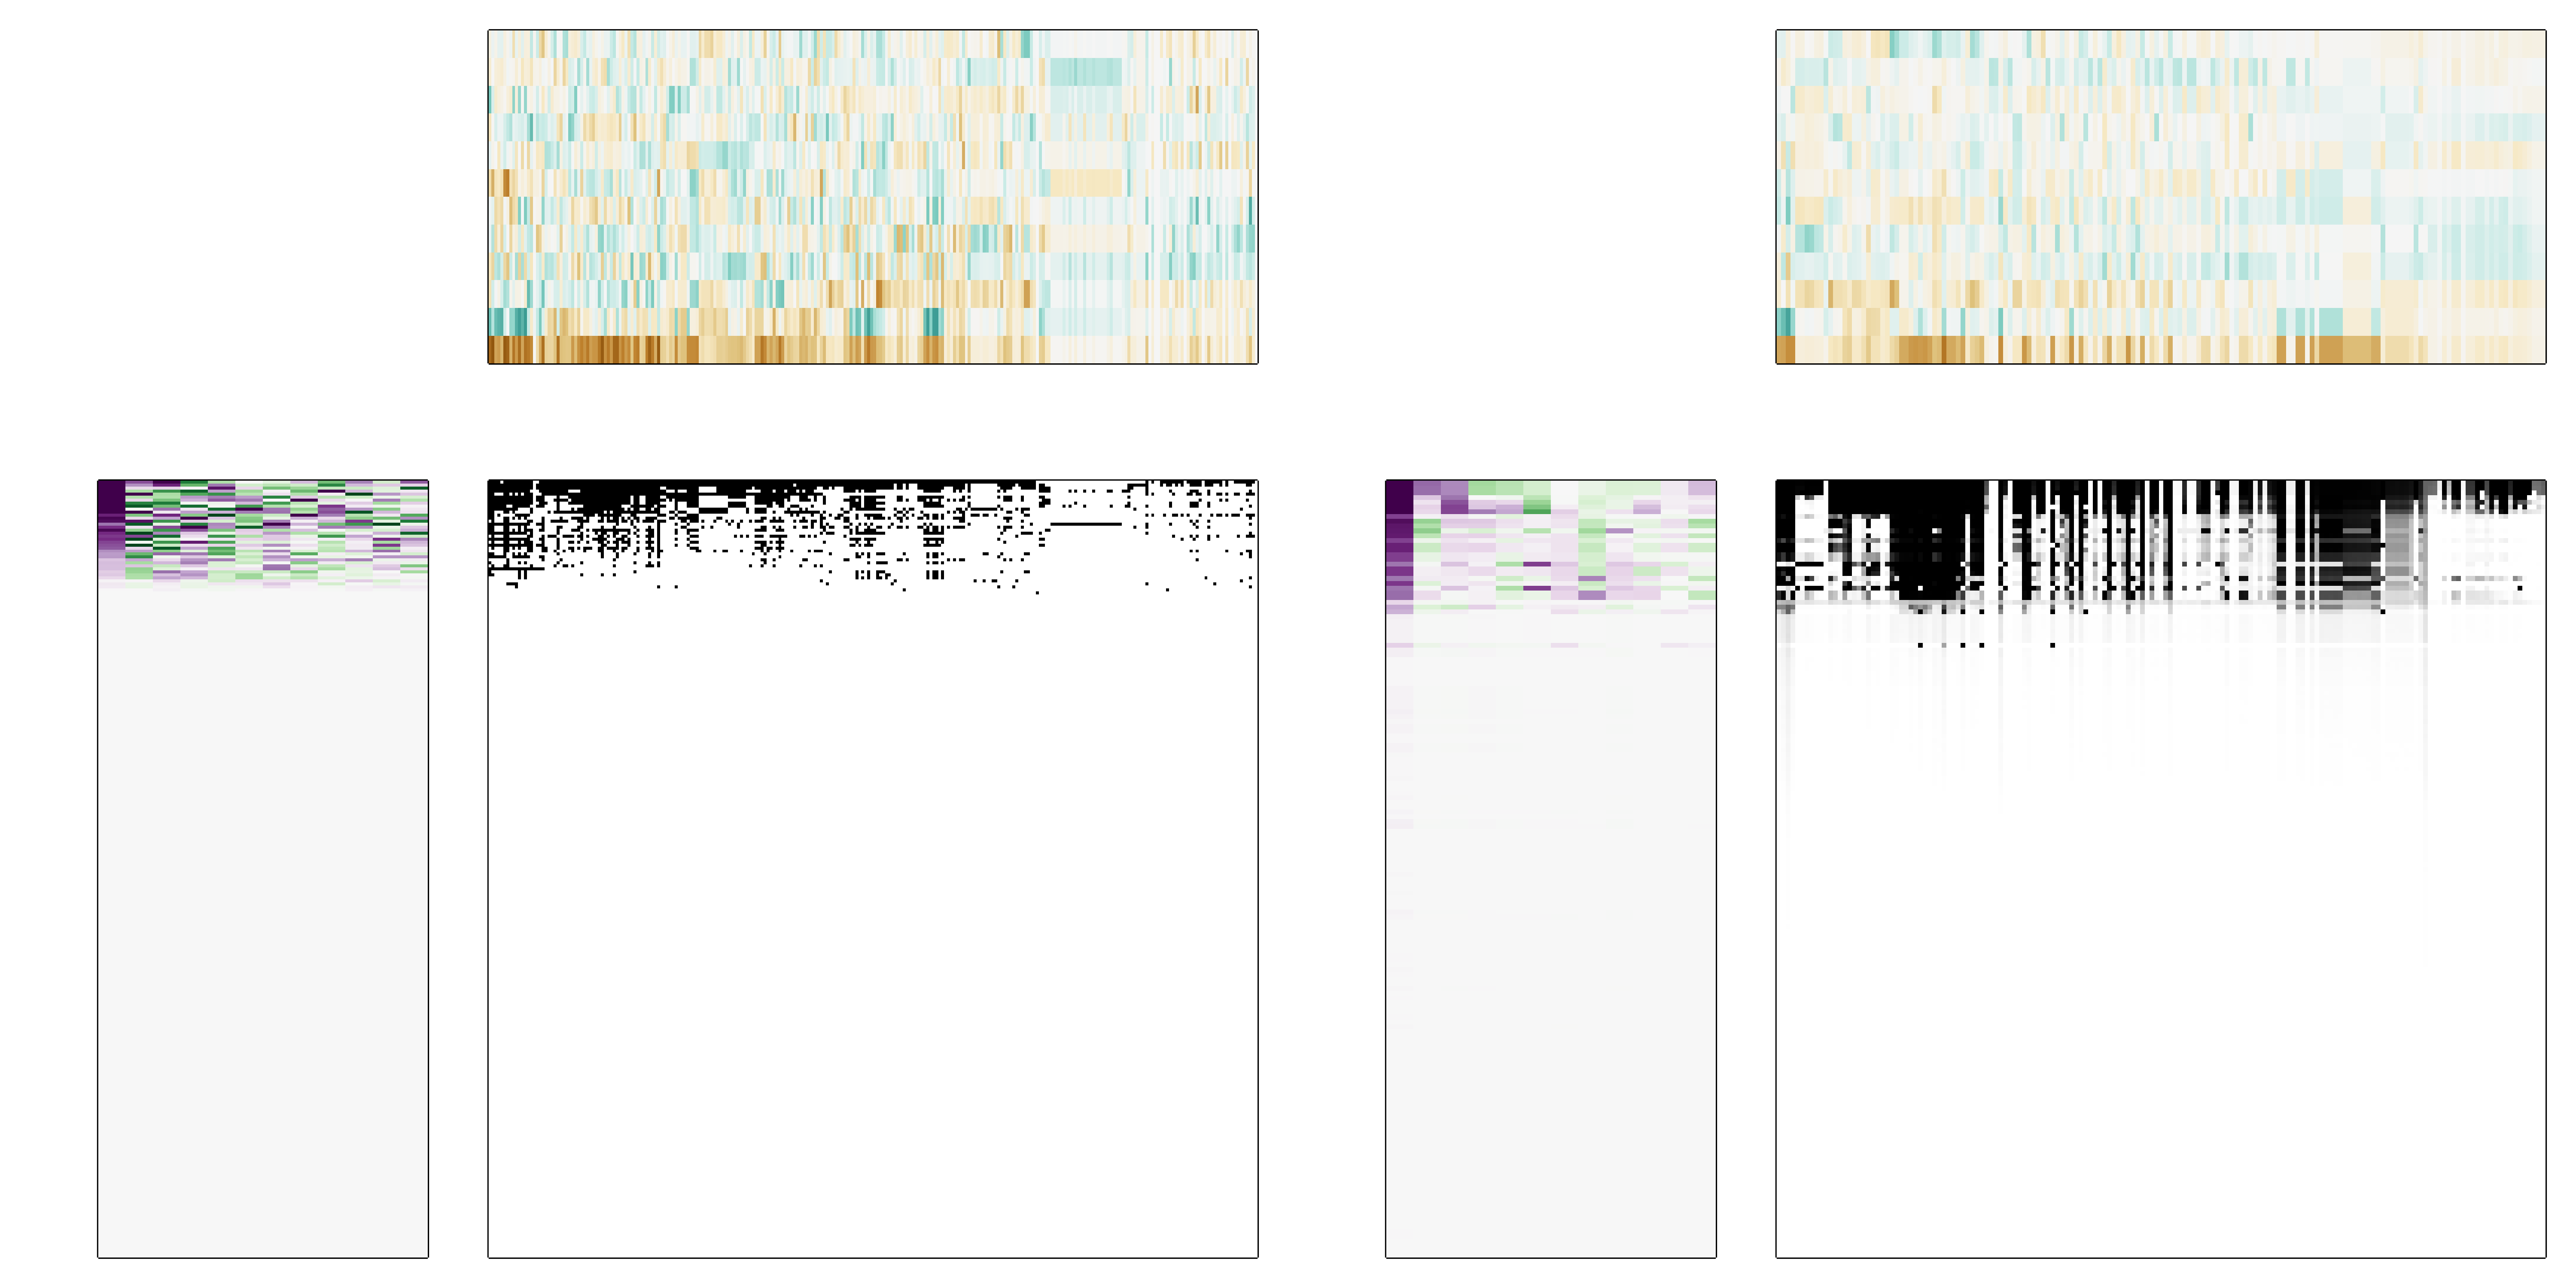
\includegraphics{figures/figure-subspaces.png}
\caption{Visual representation of the left (green/purple) and right
(green/brown) subspaces, alongside the adjacency matrix of the food web
they encode (greyscale). The European metaweb is on the left, and the
imputed Canadian metaweb (before data inflation) on the right. This
figure illustrates how much structure the left sub-space captures. As we
show in fig.~\ref{fig:degree}, the species with a value of 0 in the left
subspace are species without any prey.}\label{fig:subspaces}
}
\end{figure}

Specifically, we have adopted the following approach. For every entry in
\(\hat{\mathcal{L}}\) and \(\hat{\mathcal{R}}\), we draw a value from
its distribution. This results in one instance of the possible left
(\(\hat{\mathcal{l}}\)) and right (\(\hat{\mathcal{r}}\)) subspaces for
the Canadian metaweb. These can be multiplied, to produce one matrix of
real values. Because the entries in \(\hat{\mathcal{l}}\) and
\(\hat{\mathcal{r}}\) are in the same space where \(\mathcal{L}\) and
\(\mathcal{R}\) were originally predicted, it follows that the threshold
\(\rho\) estimated for the European metaweb also applies. We use this
information to produce one random Canadian metaweb,
\(N = \hat{\mathcal{L}}\)\(\hat{\mathcal{R}}' \ge \rho\). As we can see
in (fig.~\ref{fig:subspaces}) the European and Canadian metawebs are
structurally similar (as would be expected given the biogeographic
similarities) and the two (left and right) subspaces are distinct
\emph{i.e.} capturing predation (generality) and prey (vulnerability)
traits.

Because the intervals around some trait values can be broad (in fact,
probably broader than what they would actually be, see \emph{e.g.}
Garland \emph{et al.} 1999), we repeat the above process
\(2\times 10^5\) times, which results in a probabilistic metaweb \(P\),
where the probability of an interaction (here conveying our degree of
trust that it exists given the inferred trait distributions) is given by
the number of times where it appears across all random draws \(N\),
divided by the number of samples. An interaction with \(P_{i,j} = 1\)
means that these two species were predicted to interact in all
\(2\times 10^5\) random draws.

\hypertarget{data-cleanup-discovery-validation-and-thresholding}{%
\subsection{Data cleanup, discovery, validation, and
thresholding}\label{data-cleanup-discovery-validation-and-thresholding}}

Once the probabilistic metaweb for Canada has been produced, we followed
a number of data inflation steps to finalize it. This step is external
to the actual transfer learning framework but rather serves as a way to
augment and validate the predicted metaweb.

\begin{figure}
\hypertarget{fig:inflation}{%
\centering
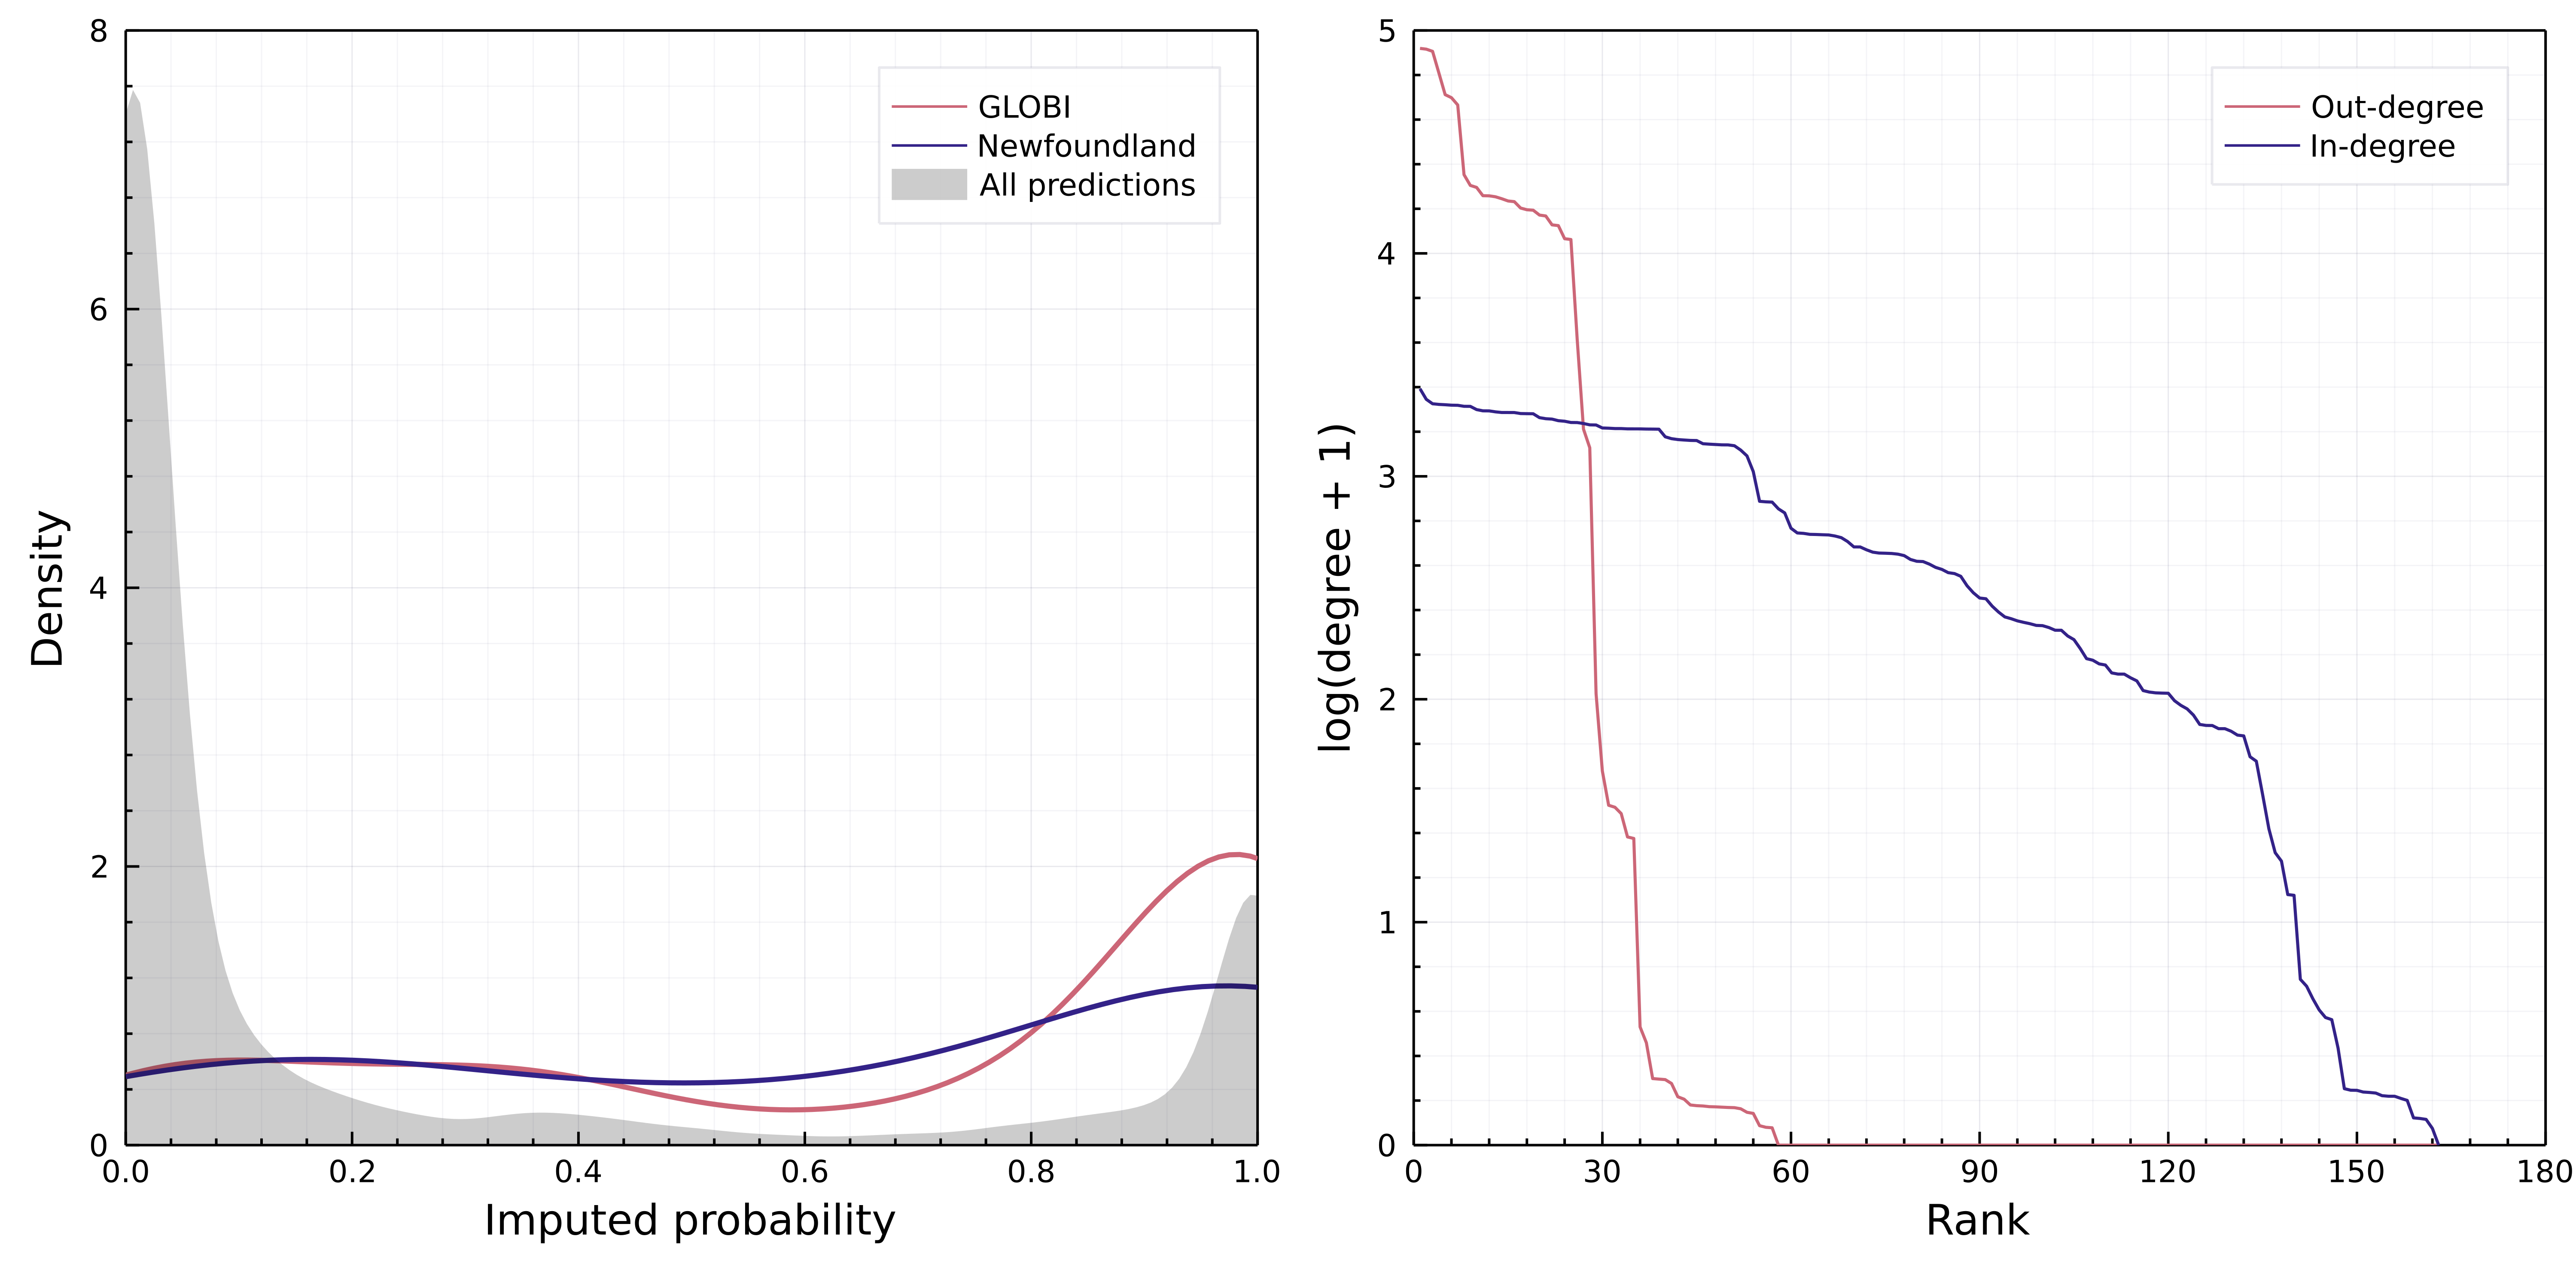
\includegraphics{figures/figure-validation.png}
\caption{Left, comparison of the probabilities of interactions assigned
by the model to all interactions (grey curve), the subset of
interactions found in GLOBI (red), and in the Strong \& Leroux (2014)
Newfoundland dataset (blue). The model recovers more interaction with a
low probability compared to data mining, which can suggest that
collected datasets are biased towards more common or easy to identify
interactions. Right, distribution of the in-degree and out-degree of the
mammals from Canada in the reconstructed metaweb. This figure describes
a flat, relatively short food web, in which there are few predators but
a large number of preys.}\label{fig:inflation}
}
\end{figure}

First, we extracted the subgraph corresponding to the 17 species shared
between the European and Canadian pools and replaced these interactions
with a probability of 0 (non-interaction) or 1 (interaction), according
to their value in the European metaweb. This represents a minute
modification of the inferred network (about 0.8\% of all species pairs
from the Canadian web), but ensures that we are directly re-using
knowledge from Europe.

Second, we looked for all species in the Canadian pool known to the
Global Biotic Interactions (GLoBI) database (Poelen \emph{et al.} 2014),
and extracted their known interactions. Because GLOBI aggregates
observed interactions, it is not a \emph{networks} data source, and
therefore the only information we can reliably extract from it is that a
species pair \emph{was reported to interact at least once}. This last
statement should yet be taken with caution, as some sources in GLOBI
(\emph{e.g.} Thessen \& Parr 2014) are produced through text analysis,
and therefore may not document direct evidence of the interaction.
Nevertheless, should the predictive model work, we would expect that a
majority of interactions known to GLOBI would also be predicted. After
performing this check, we set the probability of all interactions known
to GLOBI (366 in total, 33 of which were not predicted by the model, for
a success rate of 91\%) to 1.

Finally, we downloaded the data from Strong \& Leroux (2014), who mined
various literature sources to identify trophic interactions in
Newfoundland. This dataset documented 25 interactions between mammals,
only two of which were not part of our (Canada-level) predictions,
resulting in a success rate of 92\%. These two interactions were added
to our predicted metaweb with a probability of 1.

\begin{figure}
\hypertarget{fig:thresholds}{%
\centering
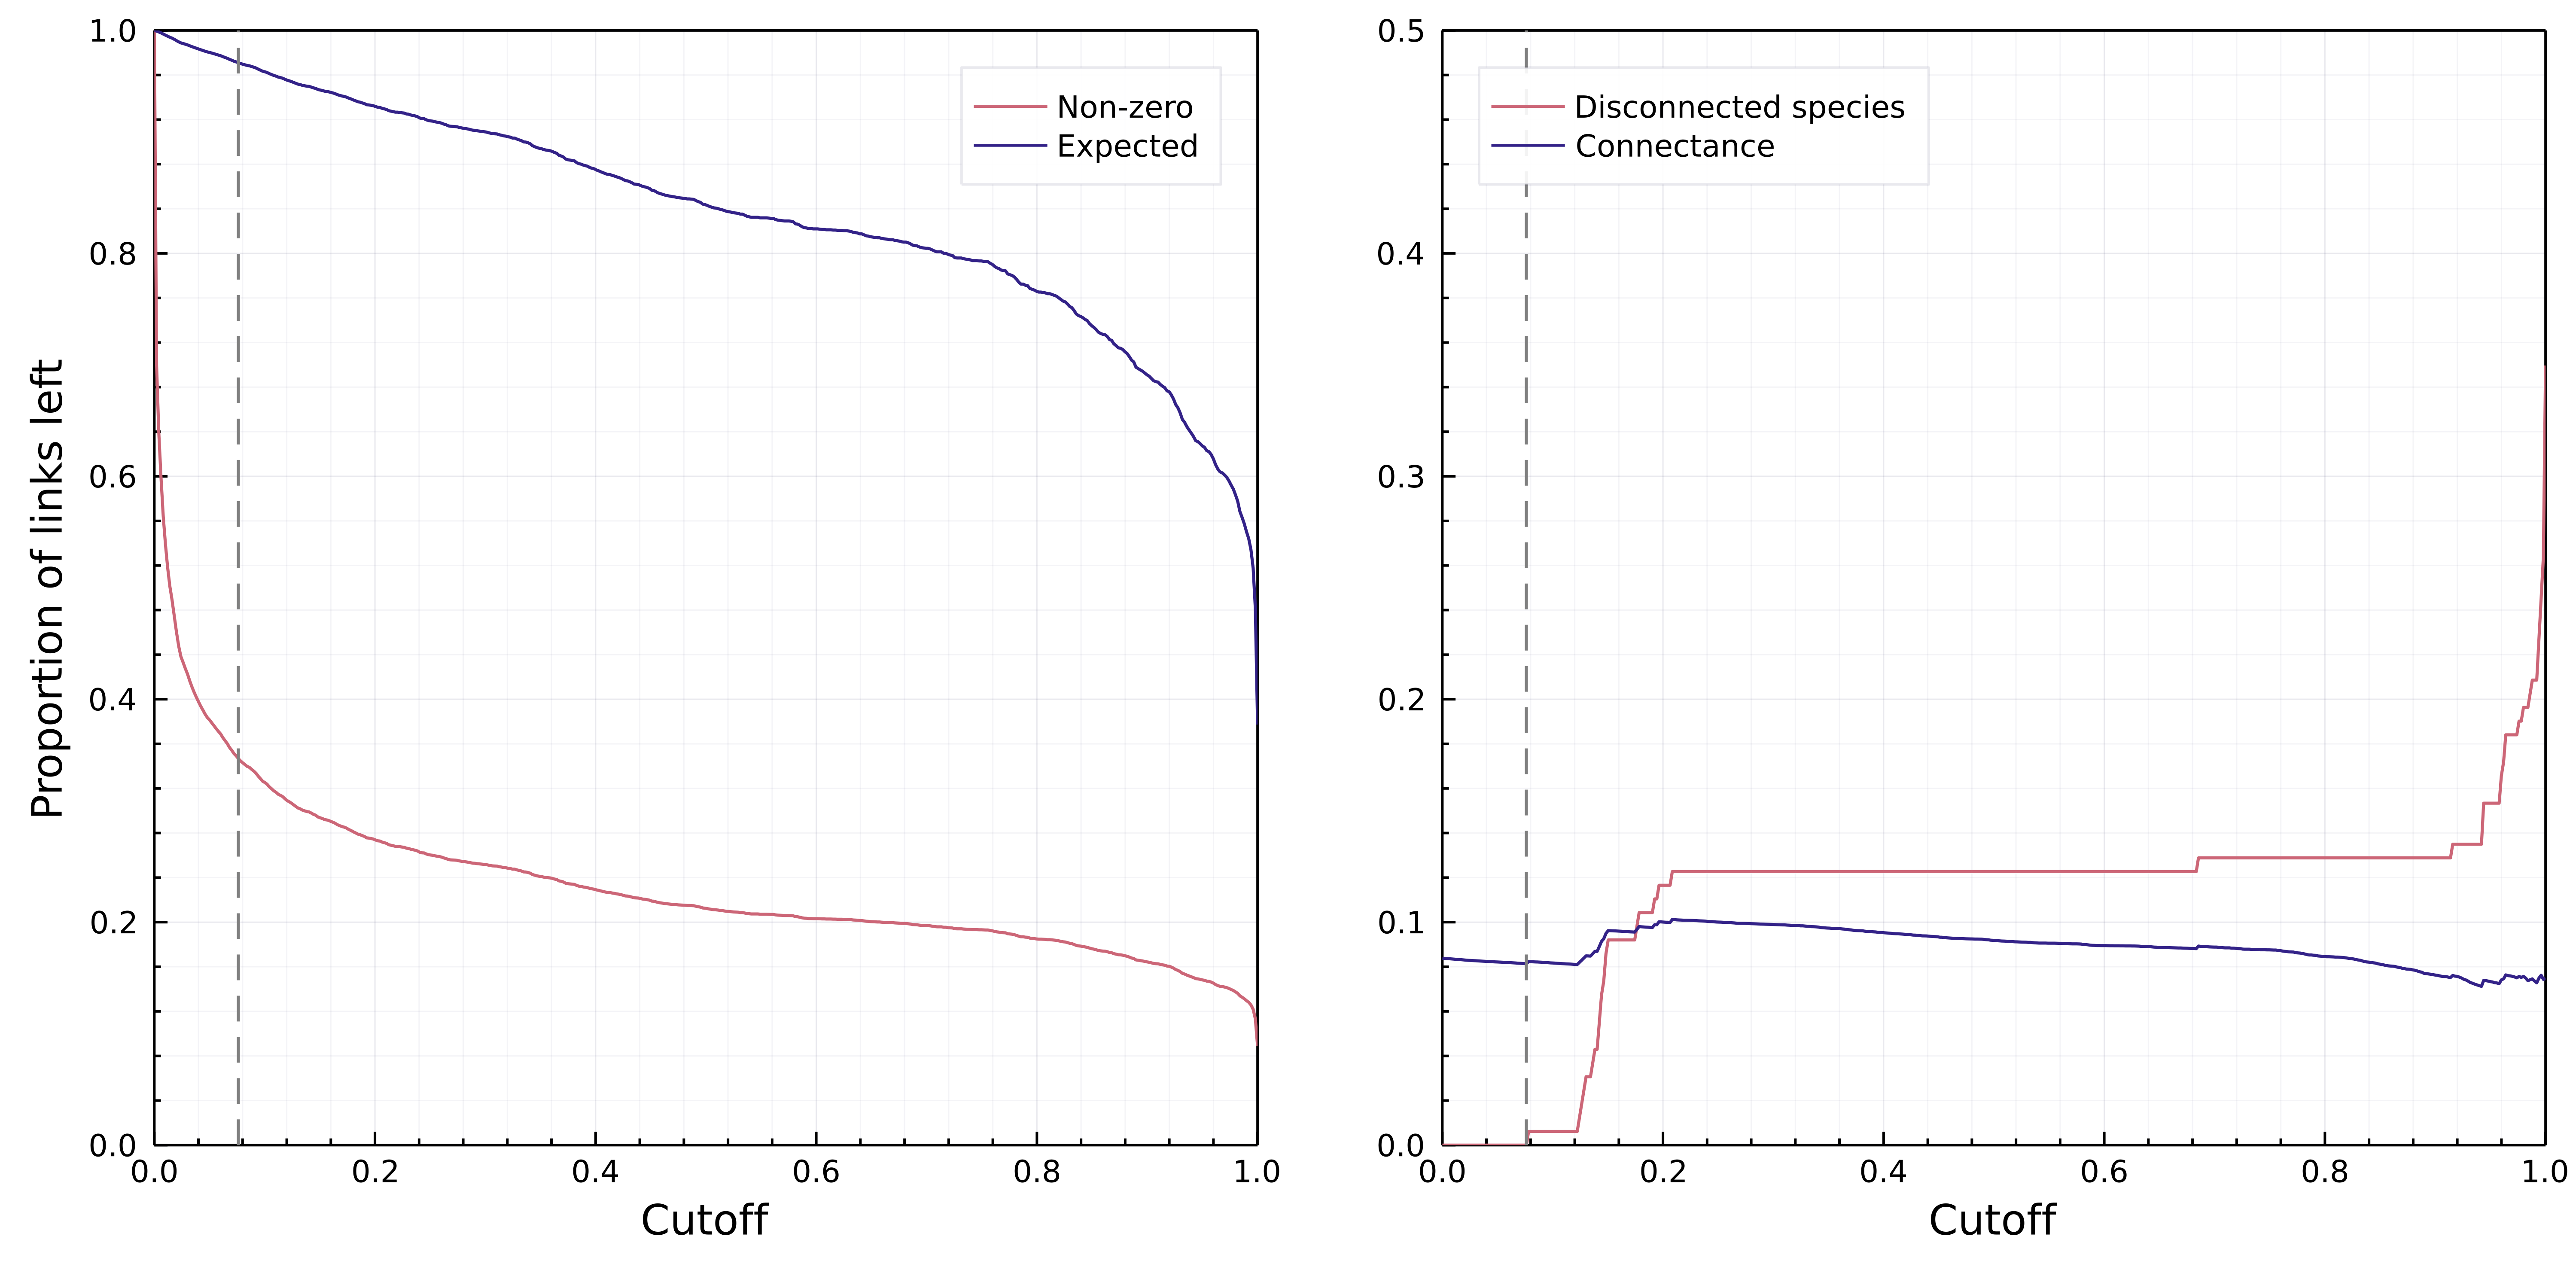
\includegraphics{figures/figure-cutoffs.png}
\caption{Left: effect of varying the cutoff for probabilities to be
considered non-zero on the number of unique links and on \(\hat{L}\),
the probabilistic estimate of the number of links assuming that all
interactions are independent. Right: effect of varying the cutoff on the
number of disconnected species, and on network connectance. In both
panels, the grey line indicates the cutoff
\(P(i\rightarrow j) \approx 0.08\) that resulted in the first species
losing all of its interactions.}\label{fig:thresholds}
}
\end{figure}

Because the confidence intervals on the inferred trait space are
probably over-estimates, we decided to apply a thresholding step to the
interactions after the data inflation (fig.~\ref{fig:thresholds}).
Cirtwill \& Hambäck (2021) proposed a number of strategies to threshold
probabilistic networks. Their methods assume the underlying data to be
tag-based sequencing, which represents interactions as co-occurrences of
predator and prey within the same tags; this is conceptually identical
to our Bernoulli-trial based reconstruction of a probabilistic network.
We performed a full analysis of the effect of various cutoffs, and as
they either resulted in removing too few interactions, or removing
enough interactions that species started to be disconnected from the
network, we set this threshold for a probability equivalent to 0 to the
largest possible value that still allowed all species to have at least
one interaction with a non-zero probability. The need for this slight
deviation from the Cirtwill \& Hambäck (2021) method highlights the need
for additional development on network thresholding.

\hypertarget{results-and-discussion-of-the-case-study}{%
\section{Results and discussion of the case
study}\label{results-and-discussion-of-the-case-study}}

In fig.~\ref{fig:thresholds}, we examine the effect of varying the
cutoff on \(P(i \rightarrow j)\) on the number of links, species, and
connectance. Determining a cutoff using the maximum curvature, or
central difference approximation of the second order partial derivative,
as suggested by \emph{e.g.} Cirtwill \& Hambäck (2021), results in
species being lost, or almost all links being kept. We therefore settled
on the value that allowed all species to remain with at least one
interaction. This result, in and of itself, suggests that additional
methodological developments for the thresholding of probabilistic
networks are required.

\begin{figure}
\hypertarget{fig:degree}{%
\centering
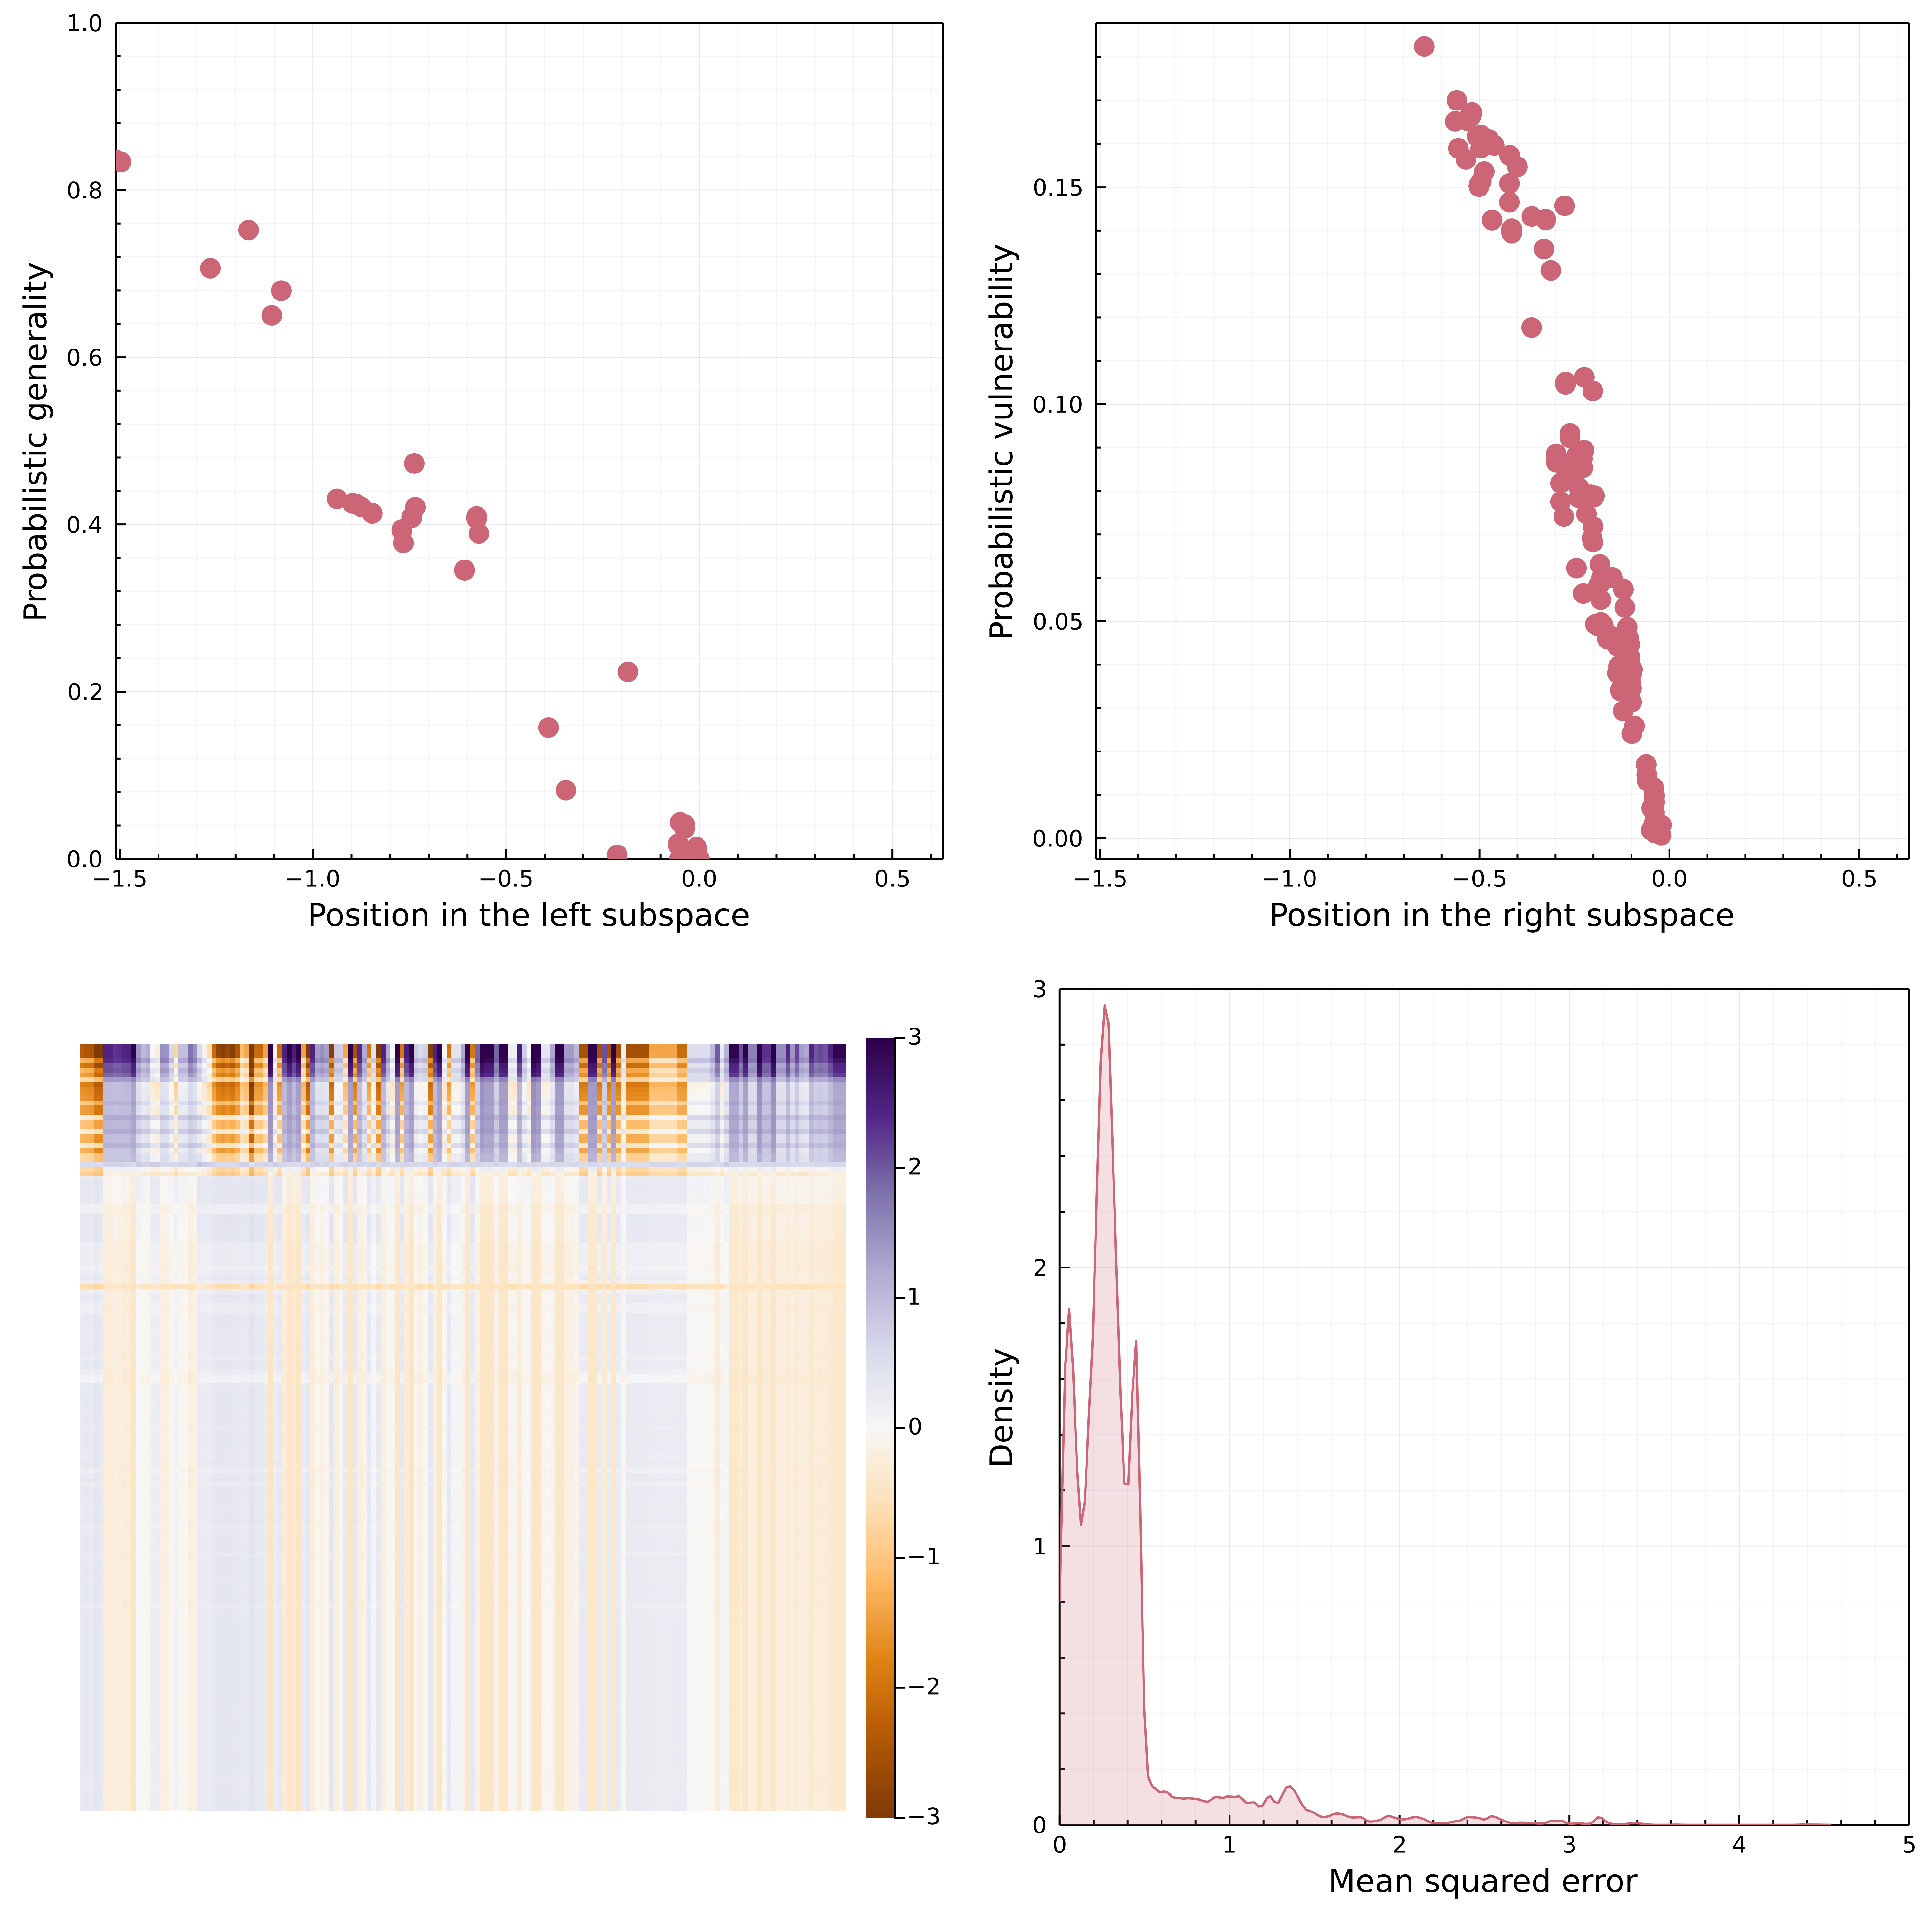
\includegraphics{figures/figure-degree.png}
\caption{Top: biological significance of the first dimension. Left:
there is a linear relationship between the values on the first dimension
of the left subspace and the generality, \emph{i.e.} the relative number
of preys, \emph{sensu} Schoener (1989). Species with a value of 0 in
this subspace are at the bottom-most trophic level. Right: there is,
similarly, a linear relationship between the position of a species on
the first dimension of the right subspace and its vulnerability,
\emph{i.e.} the relative number of predators. Taken together, these two
figures show that the first-order representation of this network would
capture its degree distribution. Bottom: topological consequences of the
first dimension. Left: differences in the \(z\)-score of the actual
configuration model for the reconstructed network, and the prediction
based only on the first dimension. Right: distribution of the
differences in the left panel.}\label{fig:degree}
}
\end{figure}

The t-SVD embedding is able to learn relevant ecological features for
the network. fig.~\ref{fig:degree} shows that the first rank correlates
linearly with generality and vulnerability (Schoener 1989), \emph{i.e.}
the number of preys and predators. Importantly, this implies that a rank
1 approximation represents the configuration model for the metaweb,
\emph{i.e.} a set of random networks generated from a given degree
sequence (Park \& Newman 2004). Accounting for the probabilistic nature
of the degrees, the rank 1 approximation also represents the \emph{soft}
configuration model (van der Hoorn \emph{et al.} 2018). Both models are
maximum entropy graph models (Garlaschelli \emph{et al.} 2018), with
sharp (all network realizations satisfy the specified degree sequence)
and soft (network realizations satisfy the degree sequence on average)
local constraints, respectively. The (soft) configuration model is an
unbiased random graph model widely used by ecologists in the context of
null hypothesis significance testing of network structure (\emph{e.g.}
Bascompte \emph{et al.} 2003) and can provide informative priors for
Bayesian inference of network structure (\emph{e.g.} Young \emph{et al.}
2021). It is noteworthy that for this metaweb, the relevant information
was extracted at the first rank. Because the first rank corresponds to
the leading singular value of the system, the results of
fig.~\ref{fig:degree} have a straightforward interpretation:
degree-based processes are the most important in structuring the
mammalian food web.

\hypertarget{discussion}{%
\section{Discussion}\label{discussion}}

One important aspect in which Europe and Canada differ (despite their
comparable bioclimatic conditions) is the degree of the legacy of human
impacts, which have been much longer in Europe. Nenzén \emph{et al.}
(2014) showed that even at small scales (the Iberian peninsula), mammal
food webs retain the signal of both climate change and human activity,
even when this human activity was orders of magnitude less important
than it is now. Similarly, Yeakel \emph{et al.} (2014) showed that
changes in human occupation over several centuries can lead to food web
collapse. Megafauna in particular seems to be very sensitive to human
arrival (Pires \emph{et al.} 2015). In short, there is
well-substantiated support for the idea that human footprint affects
more than the risk of species extinction (Marco \emph{et al.} 2018), and
can lead to changes in interaction structure. Yet, owing to the inherent
plasticity of interactions, there have been documented instances of food
webs undergoing rapid collapse/recovery cycles over short periods of
time (Pedersen \emph{et al.} 2017). The embedding of a network, in a
sense, embeds its macro-evolutionary history, especially as RDPG
captures ecological signal (Dalla Riva \& Stouffer 2016); at this point,
it is important to recall that a metaweb is intended as a catalogue of
all possible interactions, which should then be filtered
(Morales-Castilla \emph{et al.} 2015). In practice (and in this
instance) the reconstructed metaweb will predict interactions that are
plausible based on the species' evolutionary history, however some
interactions would not be realized due to human impact.

Cirtwill \emph{et al.} (2019) previously made the point that network
inference techniques based on Bayesian approaches would perform far
better in the presence of an interaction-level informative prior; the
desirable properties of such a prior would be that it is expressed as a
probability, preferably representing a Bernoulli event, the value of
which would be representative of relevant biological processes
(probability of predation in this case). We argue that the probability
returned at the very last step of our framework may serve as this
informative prior; indeed, the output of our analysis can be used in
subsequent steps, also possibly involving expert elicitation to validate
some of the most strongly recommended interactions. One important
\emph{caveat} to keep in mind when working with interaction inference is
that interactions can never really be true negatives (in the current
state of our methodological framework and data collection limitations);
this renders the task of validating a model through the usual
application of binary classification statistics very difficult (although
see Strydom \emph{et al.} 2021a for a discussion of alternative
suggestions). The other way through which our framework can be improved
is by substituting the predictors that are used for transfer. For
example, in the presence of information on species traits that are known
to be predictive of species interactions, one might want to rely on
functional rather than phylogenetic distances -- in food webs, body size
(and allometrically related variables) has been established as such a
variable (Brose \emph{et al.} 2006); the identification of relevant
functional traits is facilitated by recent methodological developments
(Rosado \emph{et al.} 2013). It should be noted that Xing \& Fayle
(2021) highlight phylogenetic relatedness as one of the core components
of network comparison at the global scale. In this case study, we have
embedded the original metaweb using t-SVD, because it lends itself to a
RDPG reconstruction, which is known to capture the consequences of
evolutionary processes (Dalla Riva \& Stouffer 2016); this being said,
there are others ways to embed graphs (Cai \emph{et al.} 2017; Arsov \&
Mirceva 2019; Cao \emph{et al.} 2019), which can be used as
alternatives.

As Herbert (1965) rightfully pointed out, ``{[}y{]}ou can't draw neat
lines around planet-wide problems''; in this regard, our approach must
contend with two interesting problems. The first is the limit of the
metaweb to embed and transfer. If the initial metaweb is too narrow in
scope, notably from a taxonomic point of view, the chances of finding
another area with enough related species to make a reliable inference
decrease. This is notably true if the metaweb is assembled in an area
with mostly endemic species. Conversely, the metaweb should be reliably
filled, which assumes that the \(S^2\) interactions in a pool of \(S\)
species have been examined, either through literature surveys or expert
elicitation. The second problem is to determine which area should be
used to infer the new metaweb in, as this determines the species pool
that must be used. In our application, we focused on the mammals of
Canada. The upside of this approach is that information at the country
level is likely to be required by policy makers and stakeholders for
their biodiversity assessment, as each country tends to set goals at the
national level (Buxton \emph{et al.} 2021) for which quantitative
instruments are designed (Turak \emph{et al.} 2017), with specific
strategies often enacted at smaller scales (Ray \emph{et al.} 2021). Yet
these national divisions, in large parts of the world, reflect nothing
except for the legacy of settler colonialism, and operating under them
must be done under the clear realization that they contributed to the
ongoing biodiversity crisis (Adam 2014), can reinforce environmental
injustice (Choudry 2013; Domínguez \& Luoma 2020), and on Turtle Island
especially, will probably end up being replaced by Indigenous principles
of land management (Eichhorn \emph{et al.} 2019; No'kmaq \emph{et al.}
2021).

\textbf{Acknowledgements:} We acknowledge that this study was conducted
on land within the traditional unceded territory of the Saint Lawrence
Iroquoian, Anishinabewaki, Mohawk, Huron-Wendat, and Omàmiwininiwak
nations. TP, TS, DC, and LP received funding from the Canadian Institue
for Ecology \& Evolution. FB is funded by the Institut de Valorisation
des Données. TS, SB, and TP are funded by a donation from the Courtois
Foundation. CB was awarded a Mitacs Elevate Fellowship no. IT12391, in
partnership with fRI Research, and also acknowledges funding from
Alberta Innovates and the Forest Resources Improvement Association of
Alberta. M-JF acknowledges funding from NSERC Discovery Grant and NSERC
CRC. RR is funded by New Zealand's Biological Heritage Ngā Koiora Tuku
Iho National Science Challenge, administered by New Zealand Ministry of
Business, Innovation, and Employment. BM is funded by the NSERC
Alexander Graham Bell Canada Graduate Scholarship and the FRQNT master's
scholarship. LP acknowledges funding from NSERC Discovery Grant (NSERC
RGPIN-2019-05771). TP acknowledges financial support from NSERC through
the Discovery Grants and Discovery Accelerator Supplement programs.

\hypertarget{references}{%
\section*{References}\label{references}}
\addcontentsline{toc}{section}{References}

\hypertarget{refs}{}
\begin{CSLReferences}{1}{0}
\leavevmode\hypertarget{ref-Adam2014EleTre}{}%
Adam, R. (2014). \emph{Elephant treaties: The Colonial legacy of the
biodiversity crisis}. UPNE.

\leavevmode\hypertarget{ref-Albouy2019MarFis}{}%
Albouy, C., Archambault, P., Appeltans, W., Araújo, M.B., Beauchesne,
D., Cazelles, K., \emph{et al.} (2019). The marine fish food web is
globally connected. \emph{Nature Ecology \& Evolution}, 3, 1153--1161.

\leavevmode\hypertarget{ref-Arsov2019NetEmb}{}%
Arsov, N. \& Mirceva, G. (2019). Network Embedding: An Overview.
\emph{arXiv:1911.11726 {[}cs, stat{]}}.

\leavevmode\hypertarget{ref-Banville2021ManJl}{}%
Banville, F., Vissault, S. \& Poisot, T. (2021). Mangal.jl and
EcologicalNetworks.jl: Two complementary packages for analyzing
ecological networks in Julia. \emph{Journal of Open Source Software}, 6,
2721.

\leavevmode\hypertarget{ref-Bascompte2003NesAss}{}%
Bascompte, J., Jordano, P., Melian, C.J. \& Olesen, J.M. (2003). The
nested assembly of plant-animal mutualistic networks. \emph{Proceedings
of the National Academy of Sciences}, 100, 9383--9387.

\leavevmode\hypertarget{ref-Beckerman2006ForBio}{}%
Beckerman, A.P., Petchey, O.L. \& Warren, P.H. (2006). Foraging biology
predicts food web complexity. \emph{Proceedings of the National Academy
of Sciences}, 103, 13745--13749.

\leavevmode\hypertarget{ref-Bezanson2017JulFre}{}%
Bezanson, J., Edelman, A., Karpinski, S. \& Shah, V. (2017). Julia: A
Fresh Approach to Numerical Computing. \emph{SIAM Review}, 59, 65--98.

\leavevmode\hypertarget{ref-Boeckaerts2021PreBac}{}%
Boeckaerts, D., Stock, M., Criel, B., Gerstmans, H., De Baets, B. \&
Briers, Y. (2021). Predicting bacteriophage hosts based on sequences of
annotated receptor-binding proteins. \emph{Scientific Reports}, 11,
1467.

\leavevmode\hypertarget{ref-Braga2021PhyRec}{}%
Braga, M.P., Janz, N., Nylin, S., Ronquist, F. \& Landis, M.J. (2021).
Phylogenetic reconstruction of ancestral ecological networks through
time for pierid butterflies and their host plants. \emph{Ecology
Letters}, n/a.

\leavevmode\hypertarget{ref-Brose2006ConRes}{}%
Brose, U., Jonsson, T., Berlow, E.L., Warren, P., Banasek-Richter, C.,
Bersier, L.-F., \emph{et al.} (2006). ConsumerResource Body-Size
Relationships in Natural Food Webs. \emph{Ecology}, 87, 2411--2417.

\leavevmode\hypertarget{ref-Buxton2021KeyInf}{}%
Buxton, R.T., Bennett, J.R., Reid, A.J., Shulman, C., Cooke, S.J.,
Francis, C.M., \emph{et al.} (2021). Key information needs to move from
knowledge to action for biodiversity conservation in Canada.
\emph{Biological Conservation}, 256, 108983.

\leavevmode\hypertarget{ref-Cai2017ComSur}{}%
Cai, H., Zheng, V.W. \& Chang, K.C.-C. (2017). A Comprehensive Survey of
Graph Embedding: Problems, Techniques and Applications. \emph{arXiv
preprint arXiv:1709.07604}.

\leavevmode\hypertarget{ref-Cameron2019UneGlo}{}%
Cameron, E.K., Sundqvist, M.K., Keith, S.A., CaraDonna, P.J., Mousing,
E.A., Nilsson, K.A., \emph{et al.} (2019). Uneven global distribution of
food web studies under climate change. \emph{Ecosphere}, 10, e02645.

\leavevmode\hypertarget{ref-Cao2019NetEmb}{}%
Cao, R.-M., Liu, S.-Y. \& Xu, X.-K. (2019). Network embedding for link
prediction: The pitfall and improvement. \emph{Chaos: An
Interdisciplinary Journal of Nonlinear Science}, 29, 103102.

\leavevmode\hypertarget{ref-Cavender-Bares2009MerCom}{}%
Cavender-Bares, J., Kozak, K.H., Fine, P.V.A. \& Kembel, S.W. (2009).
The merging of community ecology and phylogenetic biology. \emph{Ecology
Letters}, 12, 693--715.

\leavevmode\hypertarget{ref-Choudry2013SavBio}{}%
Choudry, A. (2013). Saving biodiversity, for whom and for what?
Conservation NGOs, complicity, colonialism and conquest in an era of
capitalist globalization. In: \emph{NGOization: Complicity,
contradictions and prospects}. Bloomsbury Publishing, pp. 24--44.

\leavevmode\hypertarget{ref-Cirtwill2019QuaFra}{}%
Cirtwill, A.R., Eklf, A., Roslin, T., Wootton, K. \& Gravel, D. (2019).
A quantitative framework for investigating the reliability of empirical
network construction. \emph{Methods in Ecology and Evolution}, 0.

\leavevmode\hypertarget{ref-Cirtwill2021BuiFoo}{}%
Cirtwill, A.R. \& Hambäck, P. (2021). Building food networks from
molecular data: Bayesian or fixed-number thresholds for including links.
\emph{Basic and Applied Ecology}, 50, 67--76.

\leavevmode\hypertarget{ref-DallaRiva2016ExpEvo}{}%
Dalla Riva, G.V. \& Stouffer, D.B. (2016). Exploring the evolutionary
signature of food webs' backbones using functional traits. \emph{Oikos},
125, 446--456.

\leavevmode\hypertarget{ref-Dansereau2021SimJl}{}%
Dansereau, G. \& Poisot, T. (2021). SimpleSDMLayers.jl and GBIF.jl: A
Framework for Species Distribution Modeling in Julia. \emph{Journal of
Open Source Software}, 6, 2872.

\leavevmode\hypertarget{ref-Dominguez2020DecCon}{}%
Domínguez, L. \& Luoma, C. (2020). Decolonising Conservation Policy: How
Colonial Land and Conservation Ideologies Persist and Perpetuate
Indigenous Injustices at the Expense of the Environment. \emph{Land}, 9,
65.

\leavevmode\hypertarget{ref-Dormann2010EvoCli}{}%
Dormann, C.F., Gruber, B., Winter, M. \& Herrmann, D. (2010). Evolution
of climate niches in European mammals? \emph{Biology Letters}, 6,
229--232.

\leavevmode\hypertarget{ref-Dunne2006NetStr}{}%
Dunne, J.A. (2006). The Network Structure of Food Webs. In:
\emph{Ecological networks: Linking structure and dynamics} (eds. Dunne,
J.A. \& Pascual, M.). Oxford University Press, pp. 27--86.

\leavevmode\hypertarget{ref-Eichhorn2019SteDec}{}%
Eichhorn, M.P., Baker, K. \& Griffiths, M. (2019). Steps towards
decolonising biogeography. \emph{Frontiers of Biogeography}, 12, 1--7.

\leavevmode\hypertarget{ref-Eklof2016PhyCom}{}%
Eklöf, A. \& Stouffer, D.B. (2016). The phylogenetic component of food
web structure and intervality. \emph{Theoretical Ecology}, 9, 107--115.

\leavevmode\hypertarget{ref-Garland1999IntPhy}{}%
Garland, T., JR., Midford, P.E. \& Ives, A.R. (1999). An Introduction to
Phylogenetically Based Statistical Methods, with a New Method for
Confidence Intervals on Ancestral Values1. \emph{American Zoologist},
39, 374--388.

\leavevmode\hypertarget{ref-Garlaschelli2018CovStr}{}%
Garlaschelli, D., Hollander, F. den \& Roccaverde, A. (2018). Covariance
structure behind breaking of ensemble equivalence in random graphs.
\emph{Journal of Statistical Physics}, 173, 644--662.

\leavevmode\hypertarget{ref-GBIFSecretariat2021GbiBac}{}%
GBIF Secretariat. (2021). GBIF Backbone Taxonomy.

\leavevmode\hypertarget{ref-Gerhold2015PhyPat}{}%
Gerhold, P., Cahill, J.F., Winter, M., Bartish, I.V. \& Prinzing, A.
(2015). Phylogenetic patterns are not proxies of community assembly
mechanisms (they are far better). \emph{Functional Ecology}, 29,
600--614.

\leavevmode\hypertarget{ref-Grenie2021HarTax}{}%
Grenié, M., Berti, E., Carvajal-Quintero, J.D., Winter, M. \& Sagouis,
A. (2021). Harmonizing taxon names in biodiversity data: A review of
tools, databases, and best practices.

\leavevmode\hypertarget{ref-Halko2011FinStr}{}%
Halko, N., Martinsson, P.G. \& Tropp, J.A. (2011). Finding Structure
with Randomness: Probabilistic Algorithms for Constructing Approximate
Matrix Decompositions. \emph{SIAM Review}, 53, 217--288.

\leavevmode\hypertarget{ref-Herbert1965Dun}{}%
Herbert, F. (1965). \emph{Dune}. First. Chilton Book Company,
Philadelphia.

\leavevmode\hypertarget{ref-Hortal2015SevSho}{}%
Hortal, J., de Bello, F., Diniz-Filho, J.A.F., Lewinsohn, T.M., Lobo,
J.M. \& Ladle, R.J. (2015). Seven Shortfalls that Beset Large-Scale
Knowledge of Biodiversity. \emph{Annual Review of Ecology, Evolution,
and Systematics}, 46, 523--549.

\leavevmode\hypertarget{ref-Hutchinson2017CopSig}{}%
Hutchinson, M.C., Cagua, E.F. \& Stouffer, D.B. (2017). Cophylogenetic
signal is detectable in pollination interactions across ecological
scales. \emph{Ecology}, n/a--n/a.

\leavevmode\hypertarget{ref-Jordano2016ChaEco}{}%
Jordano, P. (2016a). Chasing Ecological Interactions. \emph{PLOS Biol},
14, e1002559.

\leavevmode\hypertarget{ref-Jordano2016SamNet}{}%
Jordano, P. (2016b). Sampling networks of ecological interactions.
\emph{Functional Ecology}, 30, 1883--1893.

\leavevmode\hypertarget{ref-Litsios2012EffPhy}{}%
Litsios, G. \& Salamin, N. (2012). Effects of Phylogenetic Signal on
Ancestral State Reconstruction. \emph{Systematic Biology}, 61, 533--538.

\leavevmode\hypertarget{ref-Maiorano2020DatTet}{}%
Maiorano, L., Montemaggiori, A., Ficetola, G.F., O'Connor, L. \&
Thuiller, W. (2020a). Data from: Tetra-EU 1.0: A species-level trophic
meta-web of European tetrapods.

\leavevmode\hypertarget{ref-Maiorano2020TetEu}{}%
Maiorano, L., Montemaggiori, A., Ficetola, G.F., O'Connor, L. \&
Thuiller, W. (2020b). TETRA-EU 1.0: A species-level trophic metaweb of
European tetrapods. \emph{Global Ecology and Biogeography}, 29,
1452--1457.

\leavevmode\hypertarget{ref-Marco2018ChaHum}{}%
Marco, M.D., Venter, O., Possingham, H.P. \& Watson, J.E.M. (2018).
Changes in human footprint drive changes in species extinction risk.
\emph{Nature Communications}, 9, 4621.

\leavevmode\hypertarget{ref-Morales-Castilla2015InfBio}{}%
Morales-Castilla, I., Matias, M.G., Gravel, D. \& Araújo, M.B. (2015).
Inferring biotic interactions from proxies. \emph{Trends in Ecology \&
Evolution}, 30, 347--356.

\leavevmode\hypertarget{ref-Mouquet2012EcoAdv}{}%
Mouquet, N., Devictor, V., Meynard, C.N., Munoz, F., Bersier, L.-F.,
Chave, J., \emph{et al.} (2012). Ecophylogenetics: Advances and
perspectives. \emph{Biological Reviews}, 87, 769--785.

\leavevmode\hypertarget{ref-Nenzen2014Imp850}{}%
Nenzén, H.K., Montoya, D. \& Varela, S. (2014). The Impact of 850,000
Years of Climate Changes on the Structure and Dynamics of Mammal Food
Webs. \emph{PLOS ONE}, 9, e106651.

\leavevmode\hypertarget{ref-Nokmaq2021AwaSle}{}%
No'kmaq, M., Marshall, A., Beazley, K.F., Hum, J., joudry, shalan,
Papadopoulos, A., \emph{et al.} (2021). {``Awakening the sleeping
giant''}: Re-Indigenization principles for transforming biodiversity
conservation in Canada and beyond. \emph{FACETS}, 6, 839--869.

\leavevmode\hypertarget{ref-OConnor2020UnvFoo}{}%
O'Connor, L.M.J., Pollock, L.J., Braga, J., Ficetola, G.F., Maiorano,
L., Martinez-Almoyna, C., \emph{et al.} (2020). Unveiling the food webs
of tetrapods across Europe through the prism of the Eltonian niche.
\emph{Journal of Biogeography}, 47, 181--192.

\leavevmode\hypertarget{ref-Pan2010SurTra}{}%
Pan, S.J. \& Yang, Q. (2010). A Survey on Transfer Learning. \emph{IEEE
Transactions on Knowledge and Data Engineering}, 22, 1345--1359.

\leavevmode\hypertarget{ref-Park2004StaMec}{}%
Park, J. \& Newman, M.E.J. (2004). Statistical mechanics of networks.
\emph{Physical Review E}, 70, 066117.

\leavevmode\hypertarget{ref-Pedersen2017SigCol}{}%
Pedersen, E.J., Thompson, P.L., Ball, R.A., Fortin, M.-J., Gouhier,
T.C., Link, H., \emph{et al.} (2017). Signatures of the collapse and
incipient recovery of an overexploited marine ecosystem. \emph{Royal
Society Open Science}, 4, 170215.

\leavevmode\hypertarget{ref-Pires2015PleMeg}{}%
Pires, M.M., Koch, P.L., Fariña, R.A., de Aguiar, M.A.M., dos Reis, S.F.
\& Guimarães, P.R. (2015). Pleistocene megafaunal interaction networks
became more vulnerable after human arrival. \emph{Proceedings of the
Royal Society B: Biological Sciences}, 282, 20151367.

\leavevmode\hypertarget{ref-Poelen2014GloBio}{}%
Poelen, J.H., Simons, J.D. \& Mungall, C.J. (2014). Global biotic
interactions: An open infrastructure to share and analyze
species-interaction datasets. \emph{Ecological Informatics}, 24,
148--159.

\leavevmode\hypertarget{ref-Poisot2019EcoJl}{}%
Poisot, T., Belisle, Z., Hoebeke, L., Stock, M. \& Szefer, P. (2019).
EcologicalNetworks.jl - analysing ecological networks. \emph{Ecography}.

\leavevmode\hypertarget{ref-Poisot2021GloKno}{}%
Poisot, T., Bergeron, G., Cazelles, K., Dallas, T., Gravel, D.,
MacDonald, A., \emph{et al.} (2021a). Global knowledge gaps in species
interaction networks data. \emph{Journal of Biogeography}, n/a.

\leavevmode\hypertarget{ref-Poisot2012DisSpe}{}%
Poisot, T., Canard, E., Mouillot, D., Mouquet, N. \& Gravel, D. (2012).
The dissimilarity of species interaction networks. \emph{Ecology
Letters}, 15, 1353--1361.

\leavevmode\hypertarget{ref-Poisot2016StrPro}{}%
Poisot, T., Cirtwill, A.R., Cazelles, K., Gravel, D., Fortin, M.-J. \&
Stouffer, D.B. (2016). The structure of probabilistic networks.
\emph{Methods in Ecology and Evolution}, 7, 303--312.

\leavevmode\hypertarget{ref-Poisot2021ImpMam}{}%
Poisot, T., Ouellet, M.-A., Mollentze, N., Farrell, M.J., Becker, D.J.,
Albery, G.F., \emph{et al.} (2021b). Imputing the mammalian virome with
linear filtering and singular value decomposition.
\emph{arXiv:2105.14973 {[}q-bio{]}}.

\leavevmode\hypertarget{ref-Poisot2018IntRet}{}%
Poisot, T. \& Stouffer, D.B. (2018). Interactions retain the
co-phylogenetic matching that communities lost. \emph{Oikos}, 127,
230--238.

\leavevmode\hypertarget{ref-Price2003MacThe}{}%
Price, P.W. (2003). \emph{Macroevolutionary theory on macroecological
patterns}. Cambridge University Press.

\leavevmode\hypertarget{ref-Ray2021BioCri}{}%
Ray, J.C., Grimm, J. \& Olive, A. (2021). The biodiversity crisis in
Canada: Failures and challenges of federal and sub-national strategic
and legal frameworks. \emph{FACETS}, 6, 1044--1068.

\leavevmode\hypertarget{ref-Reeve2016HowPar}{}%
Reeve, R., Leinster, T., Cobbold, C.A., Thompson, J., Brummitt, N.,
Mitchell, S.N., \emph{et al.} (2016). How to partition diversity.
\emph{arXiv:1404.6520 {[}q-bio{]}}.

\leavevmode\hypertarget{ref-Rosado2013GoiBac}{}%
Rosado, B.H.P., Dias, A. \& de Mattos, E. (2013). Going Back to Basics:
Importance of Ecophysiology when Choosing Functional Traits for Studying
Communities and Ecosystems. \emph{Natureza \&
conservaç\textasciitilde ao revista brasileira de
conservaç\textasciitilde ao da natureza}, 11, 15--22.

\leavevmode\hypertarget{ref-Runghen2021ExpNod}{}%
Runghen, R., Stouffer, D.B. \& Dalla Riva, G.V. (2021). Exploiting node
metadata to predict interactions in large networks using graph embedding
and neural networks.

\leavevmode\hypertarget{ref-Schoener1989FooWeb}{}%
Schoener, T.W. (1989). Food webs from the small to the large.
\emph{Ecology}, 70, 1559--1589.

\leavevmode\hypertarget{ref-Solis-Lemus2017PhyPac}{}%
Solís-Lemus, C., Bastide, P. \& Ané, C. (2017). PhyloNetworks: A Package
for Phylogenetic Networks. \emph{Molecular Biology and Evolution}, 34,
3292--3298.

\leavevmode\hypertarget{ref-Stock2021PaiLea}{}%
Stock, M. (2021). Pairwise learning for predicting pollination
interactions based on traits and phylogeny. \emph{Ecological Modelling},
14.

\leavevmode\hypertarget{ref-Stouffer2012EvoCon}{}%
Stouffer, D.B., Sales-Pardo, M., Sirer, M.I. \& Bascompte, J. (2012).
Evolutionary Conservation of Species' Roles in Food Webs.
\emph{Science}, 335, 1489--1492.

\leavevmode\hypertarget{ref-Strong2014ImpNon}{}%
Strong, J.S. \& Leroux, S.J. (2014). Impact of Non-Native Terrestrial
Mammals on the Structure of the Terrestrial Mammal Food Web of
Newfoundland, Canada. \emph{PLOS ONE}, 9, e106264.

\leavevmode\hypertarget{ref-Strydom2021RoaPre}{}%
Strydom, T., Catchen, M.D., Banville, F., Caron, D., Dansereau, G.,
Desjardins-Proulx, P., \emph{et al.} (2021a). \emph{A Roadmap Toward
Predicting Species Interaction Networks (Across Space and Time)}
(Preprint). EcoEvoRxiv.

\leavevmode\hypertarget{ref-Strydom2021SvdEnt}{}%
Strydom, T., Dalla Riva, G.V. \& Poisot, T. (2021b). SVD Entropy Reveals
the High Complexity of Ecological Networks. \emph{Frontiers in Ecology
and Evolution}, 9.

\leavevmode\hypertarget{ref-Thessen2014KnoExt}{}%
Thessen, A.E. \& Parr, C.S. (2014). Knowledge extraction and semantic
annotation of text from the encyclopedia of life. \emph{PloS one}, 9,
e89550.

\leavevmode\hypertarget{ref-Torrey2010TraLea}{}%
Torrey, L. \& Shavlik, J. (2010). Transfer learning. In: \emph{Handbook
of research on machine learning applications and trends: Algorithms,
methods, and techniques}. IGI global, pp. 242--264.

\leavevmode\hypertarget{ref-Trojelsgaard2016EcoNet}{}%
Trøjelsgaard, K. \& Olesen, J.M. (2016). Ecological networks in motion:
Micro- and macroscopic variability across scales. \emph{Functional
Ecology}, 30, 1926--1935.

\leavevmode\hypertarget{ref-Turak2017UsiEss}{}%
Turak, E., Brazill-Boast, J., Cooney, T., Drielsma, M., DelaCruz, J.,
Dunkerley, G., \emph{et al.} (2017). Using the essential biodiversity
variables framework to measure biodiversity change at national scale.
\emph{Biological Conservation}, SI:Measures of biodiversity, 213,
264--271.

\leavevmode\hypertarget{ref-Upham2019InfMam}{}%
Upham, N.S., Esselstyn, J.A. \& Jetz, W. (2019). Inferring the mammal
tree: Species-level sets of phylogenies for questions in ecology,
evolution, and conservation. \emph{PLOS Biology}, 17, e3000494.

\leavevmode\hypertarget{ref-vanderHoorn2018SpaMax}{}%
van der Hoorn, P., Lippner, G. \& Krioukov, D. (2018). Sparse
Maximum-Entropy Random Graphs with a Given Power-Law Degree
Distribution. \emph{Journal of Statistical Physics}, 173, 806--844.

\leavevmode\hypertarget{ref-Xing2021RisEco}{}%
Xing, S. \& Fayle, T.M. (2021). The rise of ecological network
meta-analyses: Problems and prospects. \emph{Global Ecology and
Conservation}, 30, e01805.

\leavevmode\hypertarget{ref-Yeakel2014ColEco}{}%
Yeakel, J.D., Pires, M.M., Rudolf, L., Dominy, N.J., Koch, P.L.,
Guimarães, P.R., \emph{et al.} (2014). Collapse of an ecological network
in Ancient Egypt. \emph{PNAS}, 111, 14472--14477.

\leavevmode\hypertarget{ref-Youden1950IndRat}{}%
Youden, W.J. (1950). Index for rating diagnostic tests. \emph{Cancer},
3, 32--35.

\leavevmode\hypertarget{ref-Young2021BayInf}{}%
Young, J.-G., Cantwell, G.T. \& Newman, M.E.J. (2021). Bayesian
inference of network structure from unreliable data. \emph{Journal of
Complex Networks}, 8.

\leavevmode\hypertarget{ref-Young2007RanDot}{}%
Young, S.J. \& Scheinerman, E.R. (2007). Random Dot Product Graph Models
for Social Networks. In: \emph{Algorithms and Models for the Web-Graph},
Lecture Notes in Computer Science (eds. Bonato, A. \& Chung, F.R.K.).
Springer, Berlin, Heidelberg, pp. 138--149.

\leavevmode\hypertarget{ref-Zhu2006AutDim}{}%
Zhu, M. \& Ghodsi, A. (2006). Automatic dimensionality selection from
the scree plot via the use of profile likelihood. \emph{Computational
Statistics \& Data Analysis}, 51, 918--930.

\end{CSLReferences}

\end{document}
